%\documentclass[handout]{beamer}
\documentclass[]{beamer}
%\documentclass[draft]{beamer}

\mode<presentation>
{
  \usetheme{Warsaw}
  % \setbeamercovered{transparent}
  \useoutertheme{infolines}

}

\usepackage[italian]{babel}
\usepackage[utf8]{inputenc}
\usepackage{wrapfig}
\usepackage[T1]{fontenc}
\usepackage{float}
\usepackage{multicol}
\usepackage{pgfplots}
\usepackage{graphicx}
\usepackage{algorithm}
\usepackage{xcolor}
\usepackage{tikz}
\usetikzlibrary{positioning,shapes,chains,backgrounds,arrows,chains,fit,snakes,
  calc,automata}
\usepackage{array}
\usepackage{subcaption}
\pgfplotsset{compat=1.13}
\usepackage{pdfpages}
\newcolumntype{P}[1]{>{\centering\arraybackslash}p{#1}}
\usepackage{algorithm}
\usepackage[noend]{algpseudocode}
\usepackage{blindtext}
\usepackage{mwe}

\usepackage{tikz}\usetikzlibrary{er}\tikzset{multi  attribute /.style={attribute
    ,double  distance =1.5pt}}\tikzset{derived  attribute /.style={attribute
    ,dashed}}\tikzset{total /.style={double  distance =1.5pt}}\tikzset{every
  entity /.style={draw=orange , fill=orange!20}}\tikzset{every  attribute
  /.style={draw=MediumPurple1, fill=MediumPurple1!20}}\tikzset{every
  relationship /.style={draw=Chartreuse2,
    fill=Chartreuse2!20}}\newcommand{\key}[1]{\underline{#1}}
\usetikzlibrary{arrows.meta}
\usetikzlibrary{decorations.markings}
\usetikzlibrary{arrows,shapes,backgrounds,petri} 
\usetikzlibrary{automata,positioning}
\usetikzlibrary{matrix}

\definecolor{nord1}{RGB}{46, 52, 64}
\definecolor{nord2}{RGB}{76, 105, 141}
\definecolor{nord3}{RGB}{94, 129, 172}
\definecolor{nord4}{RGB}{129, 161, 193}
\definecolor{nord5}{RGB}{136, 192, 208}
\definecolor{nord6}{RGB}{163, 190, 140}
\definecolor{nord7}{RGB}{191, 97, 106}
\definecolor{nordred}{RGB}{191, 97, 106}
\definecolor{nordgreen}{RGB}{135, 157, 116}
\definecolor{nordred}{RGB}{191, 97, 106}
\definecolor{nordcyan}{RGB}{94,129,172}
\definecolor{nordgreen}{RGB}{135, 157, 116}
\definecolor{nordpurple}{RGB}{180,142,173}

\setbeamercolor{palette primary}{bg=nord2,fg=white}
\setbeamercolor{palette secondary}{bg=nord3,fg=white}
\setbeamercolor{palette tertiary}{bg=nord4,fg=white}


\setbeamercolor{block title}{bg=nord2,fg=white}

\setbeamercolor{itemize item}{fg=nord3}
\setbeamercolor{itemize subitem}{fg=nord4}
\setbeamercolor{itemize subsubitem}{fg=nord5}

\setbeamertemplate{itemize item}[square]
\setbeamertemplate{itemize subitem}[circle]
\setbeamertemplate{itemize subsubitem}[triangle]
\setbeamerfont{bibliography item}{size=\scriptsize}
\setbeamerfont{bibliography entry author}{size=\scriptsize}
\setbeamerfont{bibliography entry title}{size=\scriptsize}
\setbeamerfont{bibliography entry location}{size=\tiny}
\setbeamerfont{bibliography entry note}{size=\tiny}

\usecolortheme[named=nord2]{structure}
\setbeamertemplate{bibliography item}{\insertbiblabel}
\def\SLP{\mbox{\rm {\sf SLP}}}
\def\rank{\mbox{\rm {\sf rank}}}
\def\lcs{\mbox{\rm {\sf lcs}}}
\def\lcp{\mbox{\rm {\sf lcp}}}
\def\lce{\mbox{\rm {\sf lce}}}
\def\LCE{\mbox{\rm {\sf LCE}}}
\def\ROT{\mbox{\rm {\sf ROT}}}
\def\select{\mbox{\rm {\sf select}}}
\def\col{\mbox{\rm {\sf col}}}
\def\NULL{\mbox{\rm {\sf null}}}
\def\len{\mbox{\rm {\sf len}}}
\def\pos{\mbox{\rm {\sf pos}}}
\def\row{\mbox{\rm {\sf row}}}
\def\LF{\mbox{\rm {\sf LF}}}
\def\FL{\mbox{\rm {\sf FL}}}
\def\W{\mbox{\rm {\sf w}}}
\def\A{\mbox{\rm {\sf A}}}
\def\A{\mbox{\rm {\sf A}}}
\def\SA{\mbox{\rm {\sf SA}}}
\def\IISA{\mbox{\rm {\sf (I)SA}}}
\def\LCP{\mbox{\rm {\sf LCP}}}
\def\ISA{\mbox{\rm {\sf ISA}}}
\def\PLCP{\mbox{\rm {\sf PLCP}}}
\def\PPLCP{\mbox{\rm {\sf (P)LCP}}}

\def\RLCP{\mbox{\rm {\sf RLCP}}}
\def\RLBWT{\mbox{\rm {\sf RLBWT}}}
\def\MEM{\mbox{\rm {\sf MEM}}}
\def\KMEM{\mbox{\rm {\sf K-MEM}}}
\def\KSMEM{\mbox{\rm {\sf K-SMEM}}}
\def\MS{\mbox{\rm {\sf MS}}}
\def\LCP{\mbox{\rm {\sf LCP}}}
\def\NSV{\mbox{\rm {\sf NSV}}}
\def\PSV{\mbox{\rm {\sf PSV}}}
\def\RMQ{\mbox{\rm {\sf RMQ}}}
\def\BWT{\mbox{\rm {\sf BWT}}}
\def\BWM{\mbox{\rm {\sf BWM}}}
\def\ITR{\mbox{\rm {\sf index\_to\_run}}}
\def\GS{\mbox{\rm {\sf get\_symbol}}}
\def\PBWT{\mbox{\rm {\sf PBWT}}}
\def\MPBWT{\mbox{\rm {\sf mPBWT}}}
\def\MRLPBWT{\mbox{\rm {\sf mRLPBWT}}}
\def\DPBWT{\mbox{\rm {\sf dPBWT}}}
\def\RLPBWT{\mbox{\rm {\sf RLPBWT}}}
\def\SMEM{\mbox{\rm {\sf SMEM}}}
\def\M{\mbox{\rm {\sf M}}}
\def\C{\mbox{\rm {\sf C}}}
\def\Occ{\mbox{\rm {\sf Occ}}}
\def\L{\mbox{\rm {\sf L}}}
\def\F{\mbox{\rm {\sf F}}}
\def\DA{\mbox{\rm {\sf DA}}}
\def\DM{\mbox{\rm {\sf DM}}}
\def\PA{\mbox{\rm {\sf PA}}}
\def\LCE{\mbox{\rm {\sf LCE}}}
\def\UP{\mbox{\rm {\sf update}}}
\def\lceb{\mbox{\rm {\sf lce\_bounded}}}
\def\RM{\mbox{\rm {\sf reverse\_map}}}

\newcommand{\Oh}{\mathcal{O}}

\newcommand{\tikzmark}[1]{\tikz[overlay,remember picture] \node (#1) {};}
\newcommand{\DrawBox}[3][]{%
    \tikz[overlay,remember picture]{
    \draw[black,#1]
      ($(#2)+(-0.2em,2.0ex)$) rectangle
      ($(#3)+(0.2em,-0.5ex)$);}
  }
  
\title[Algoritmi per la $\RLPBWT$] {Algoritmi per la trasformata di
  Burrows-Wheeler posizionale con compressione run-length}

% \subtitle
% {Presentation Subtitle} % (optional)

\author[Davide Cozzi]{\Large{Davide Cozzi}}


\institute[] {\large{\textbf{{\color{nord2}Relatore:}}
    \textit{Prof.ssa~Raffaella 
      Rizzi}\quad 
    \textbf{\color{nord2}{Correlatore:}} \textit{Dr.~Yuri Pirola}}\\
  \vspace{4mm}
  \small{\textit{Dipartimento di Informatica, Sistemistica e Comunicazione
      (DISCo)\\
      Università degli Studi di Milano Bicocca}}}

\date[26/10/2022] {26 Ottobre 2022}

\subject{Presentatazione}
\pgfdeclareimage[height=0.5cm]{university-logo}{img/logo_unimib.pdf}
\logo{\pgfuseimage{university-logo}}

% \AtBeginSection[]
% {
%   \begin{frame}<beamer>{Outline}
%     \tableofcontents[currentsection, currentsubsection]
%   \end{frame}
% }


% If you wish to uncover everything in a step-wise fashion, uncomment
% the following command: 

% \beamerdefaultoverlayspecification{<+->}
\def\Cplusplus{C\raisebox{0.5ex}{\tiny\textbf{++}}}


\begin{document}
\begin{frame}
  \titlepage
\end{frame}

\begin{frame}{Outline}
  \setcounter{tocdepth}{1}
  \tableofcontents
\end{frame}
\section{Introduzione e scopo della tesi}
\subsection{Pangenoma e aplotipi}
\begin{frame}{Un punto di vista per il pangenoma}
  % \begin{block}{}
  %   \small{
  %   Negli ultimi anni si è assistito a un cambio di paradigma nel campo della
  %   \textit{bioinformatica}, ovvero il passaggio dallo studio della sequenza
  %   lineare di 
  %   un singolo genoma a quello di un insieme di genomi, provenienti da un gran
  %   numero di individui, al fine di poter considerare anche le varianti geniche.
  %   Questo nuovo concetto è stato introdotto da Tettelin, nel 2005, con il
  %   termine di \textbf{pangenoma}.}
  % \end{block}
  % \begin{block}{}
  %   \small{
  %   Uno degli approcci più usati per rappresentare il \textbf{pangenoma}
  %   è attraverso un pannello di aplotipi, ovvero, da un punto di vista
  %   computazionale, una matrice di M righe, corrispondenti agli individui, e N
  %   colonne, corrispondenti ai siti con le varianti. }
  % \end{block}
  % \begin{block}{}
  %   \small{
  %   Un \textbf{aplotipo} è  l'insieme di alleli, ovvero di
  %   varianti che, a meno di mutazioni, un organismo eredita da ogni genitore. }
  % \end{block}
  \only<1>{
    \begin{block}{Il pangenoma}
      \begin{itemize}
        \item studio di un insieme di genomi provenienti da diversi individui
        \item Studio delle varianti geniche
      \end{itemize}
    \end{block}
    \begin{block}{}
      \begin{itemize}
        \item unica sequenze per multiple sequenze lineari
        \item grafo del pangenoma
        \item \underline{\textbf{pannello di aplotipi}}
      \end{itemize}
    \end{block}
    \begin{block}{}
      Un \textbf{aplotipo} è  l'insieme di alleli, ovvero di
      varianti che, a meno di mutazioni, un organismo eredita da ogni genitore.
    \end{block}
  }\only<2>{
    \begin{figure}[H]
      \centering
      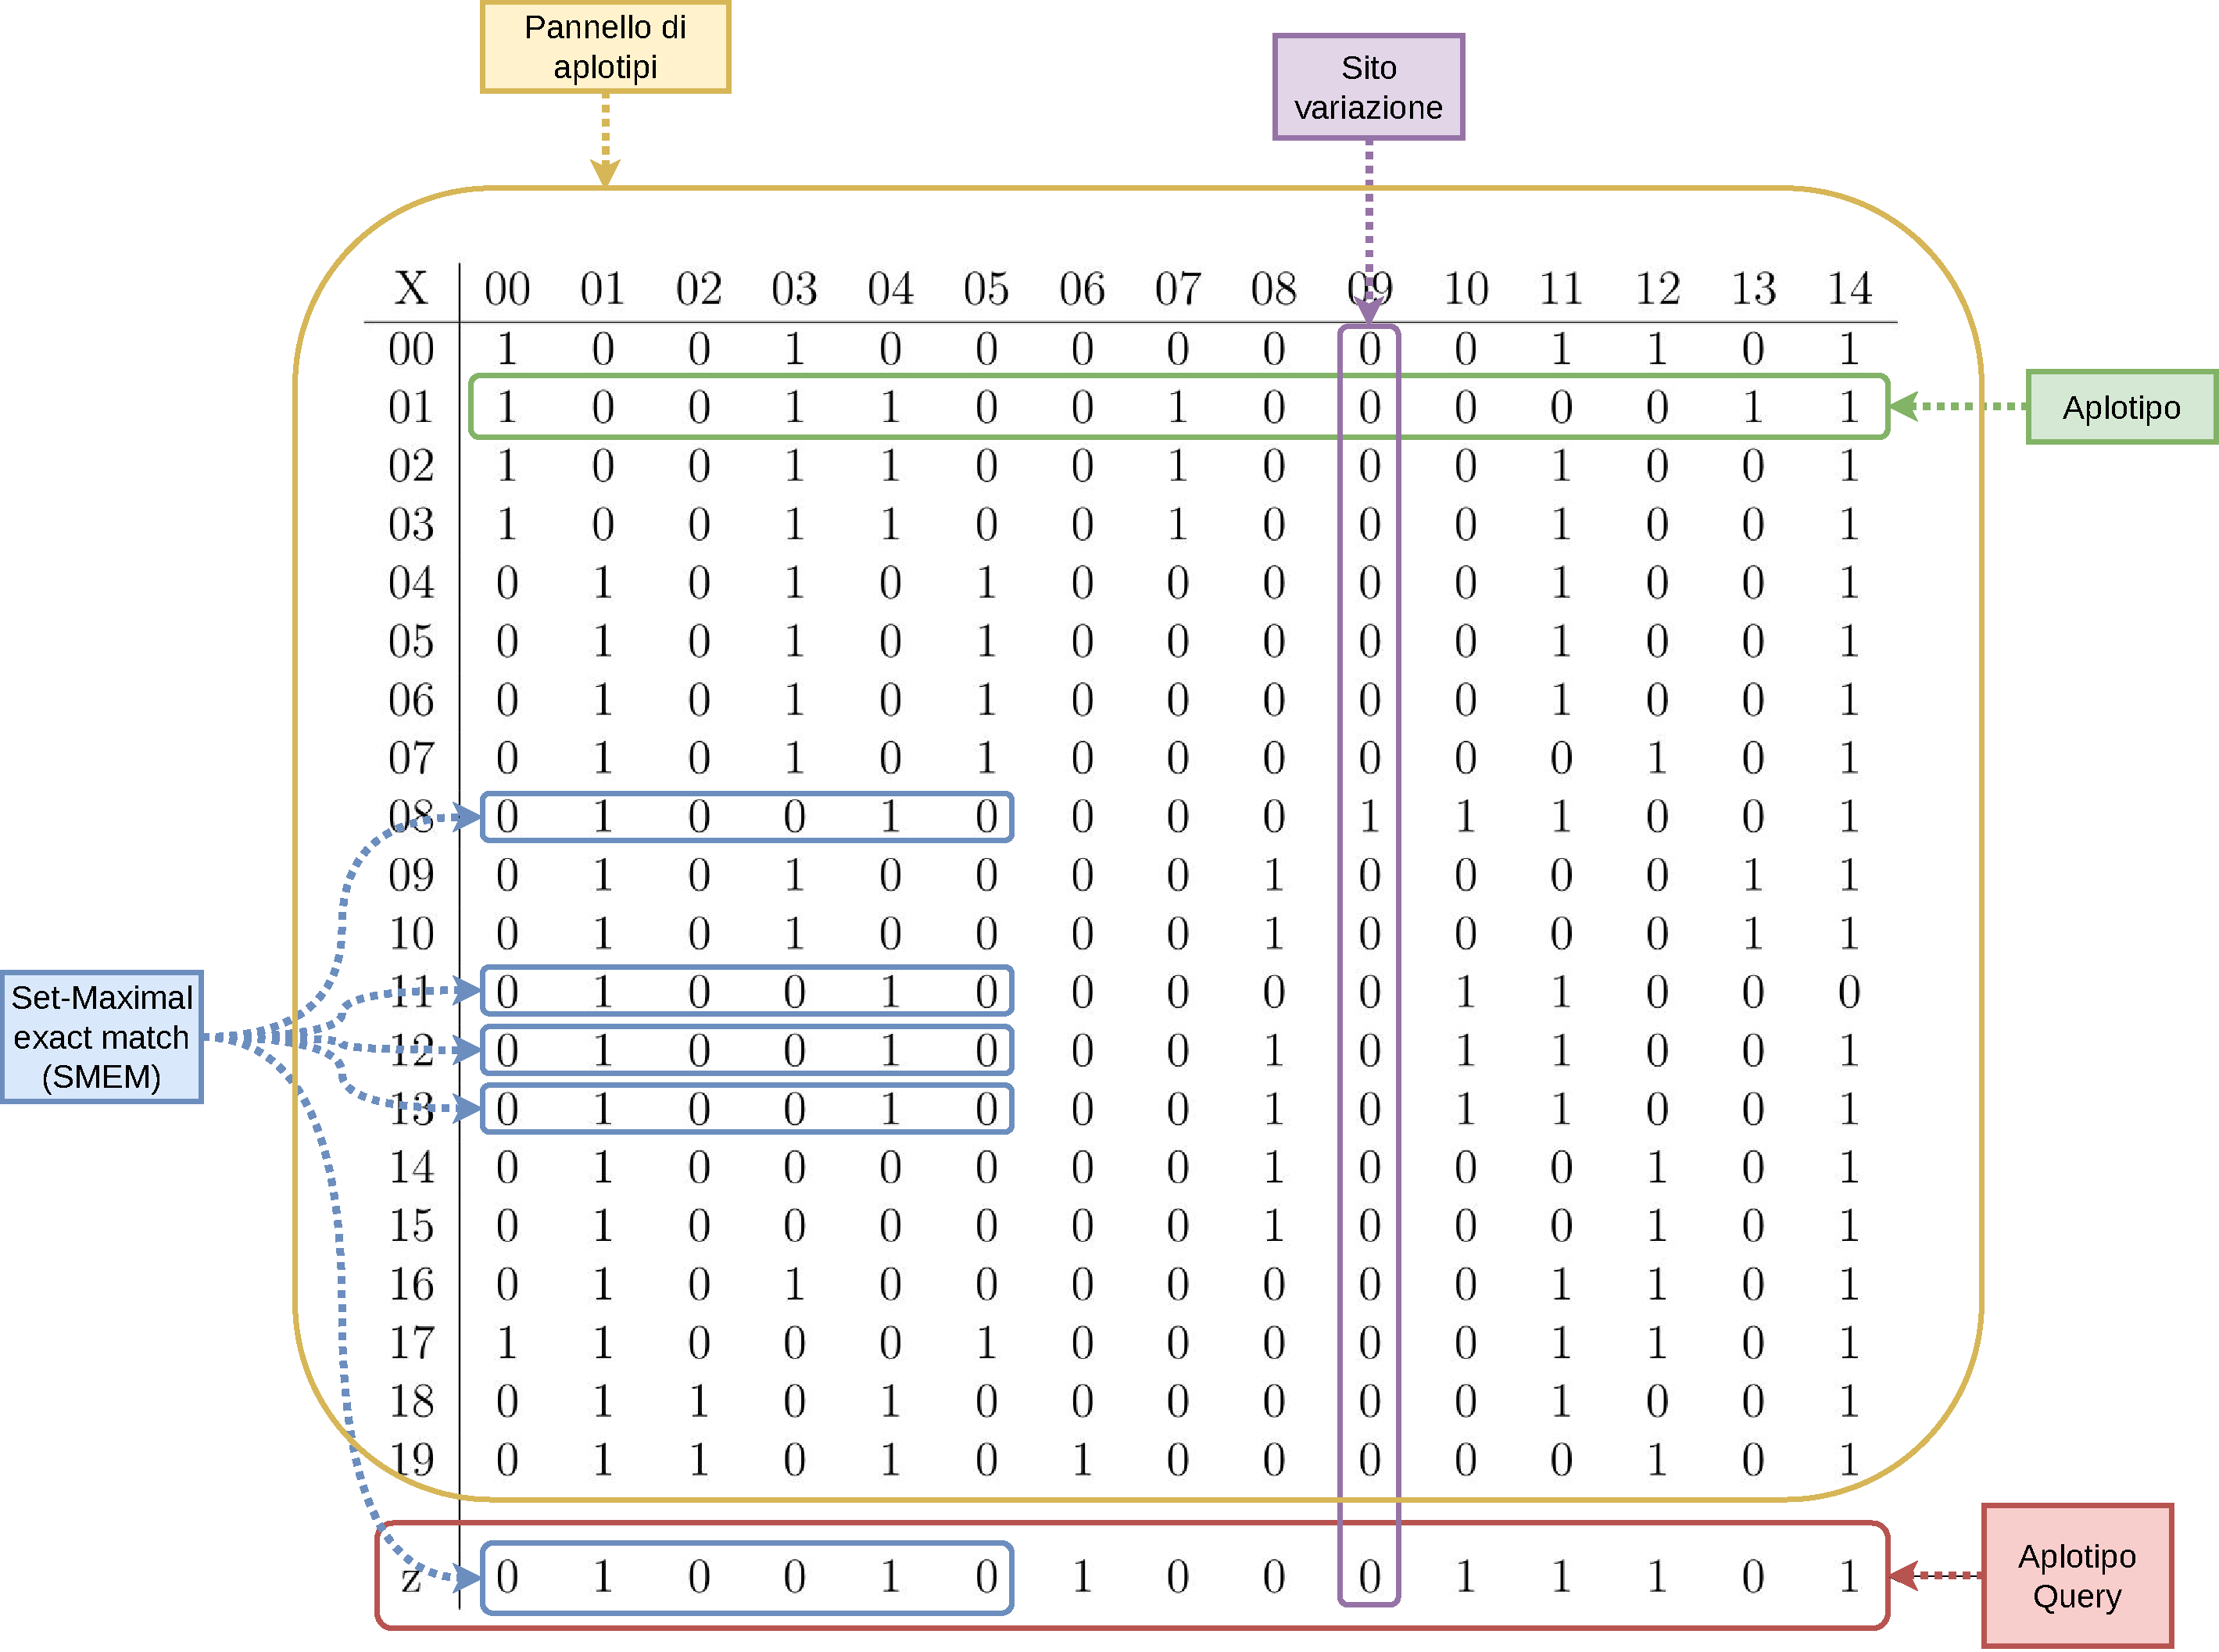
\includegraphics[width=0.85\textwidth]{img/full.pdf}
    \end{figure}
  }
\end{frame}
\begin{frame}{Trasformata di Burrows--Wheeler posizionale}
  \only<1>{
    \begin{block}{$\PBWT$ - {\footnotesize{\textit{Durbin, Bioinformatics,
              2014}}}} 
      Dato pannello di $M$ aplotipi, lunghi $N$ siti (biallelici:
      $\Sigma=\{0,1\}$), si definisce 
      $\PBWT$ del 
      pannello una collezione di $N+1$ coppie di array $(a_k,d_k)$, $0\leq k\leq
      N$, dove:
      \begin{itemize}
        \item $a_k$ è il \textbf{prefix array} della colonna $k$
        \item $d_k$ è il \textbf{divergence array} della colonna $k$
      \end{itemize}
      Il pannello, riordinato in ogni colonna $k$ con $a_k$, è detto:
      \underline{matrice $\PBWT$}. 
    \end{block}
    \begin{block}{Run-length encoding}
      Il run-length encoding consiste nel memorizzare le \textit{run}, ovvero
      sequenze massimali di caratteri uguali, come coppie: \\
      \vspace{-0.3cm}
      \begin{center}
        \texttt{(carattere, lunghezza della run)}\\
        \texttt{000000} $\implies$ \texttt{(0,6)}
      \end{center}
    \end{block}
  }\only<2>{
    \begin{figure}[H]
      \centering
      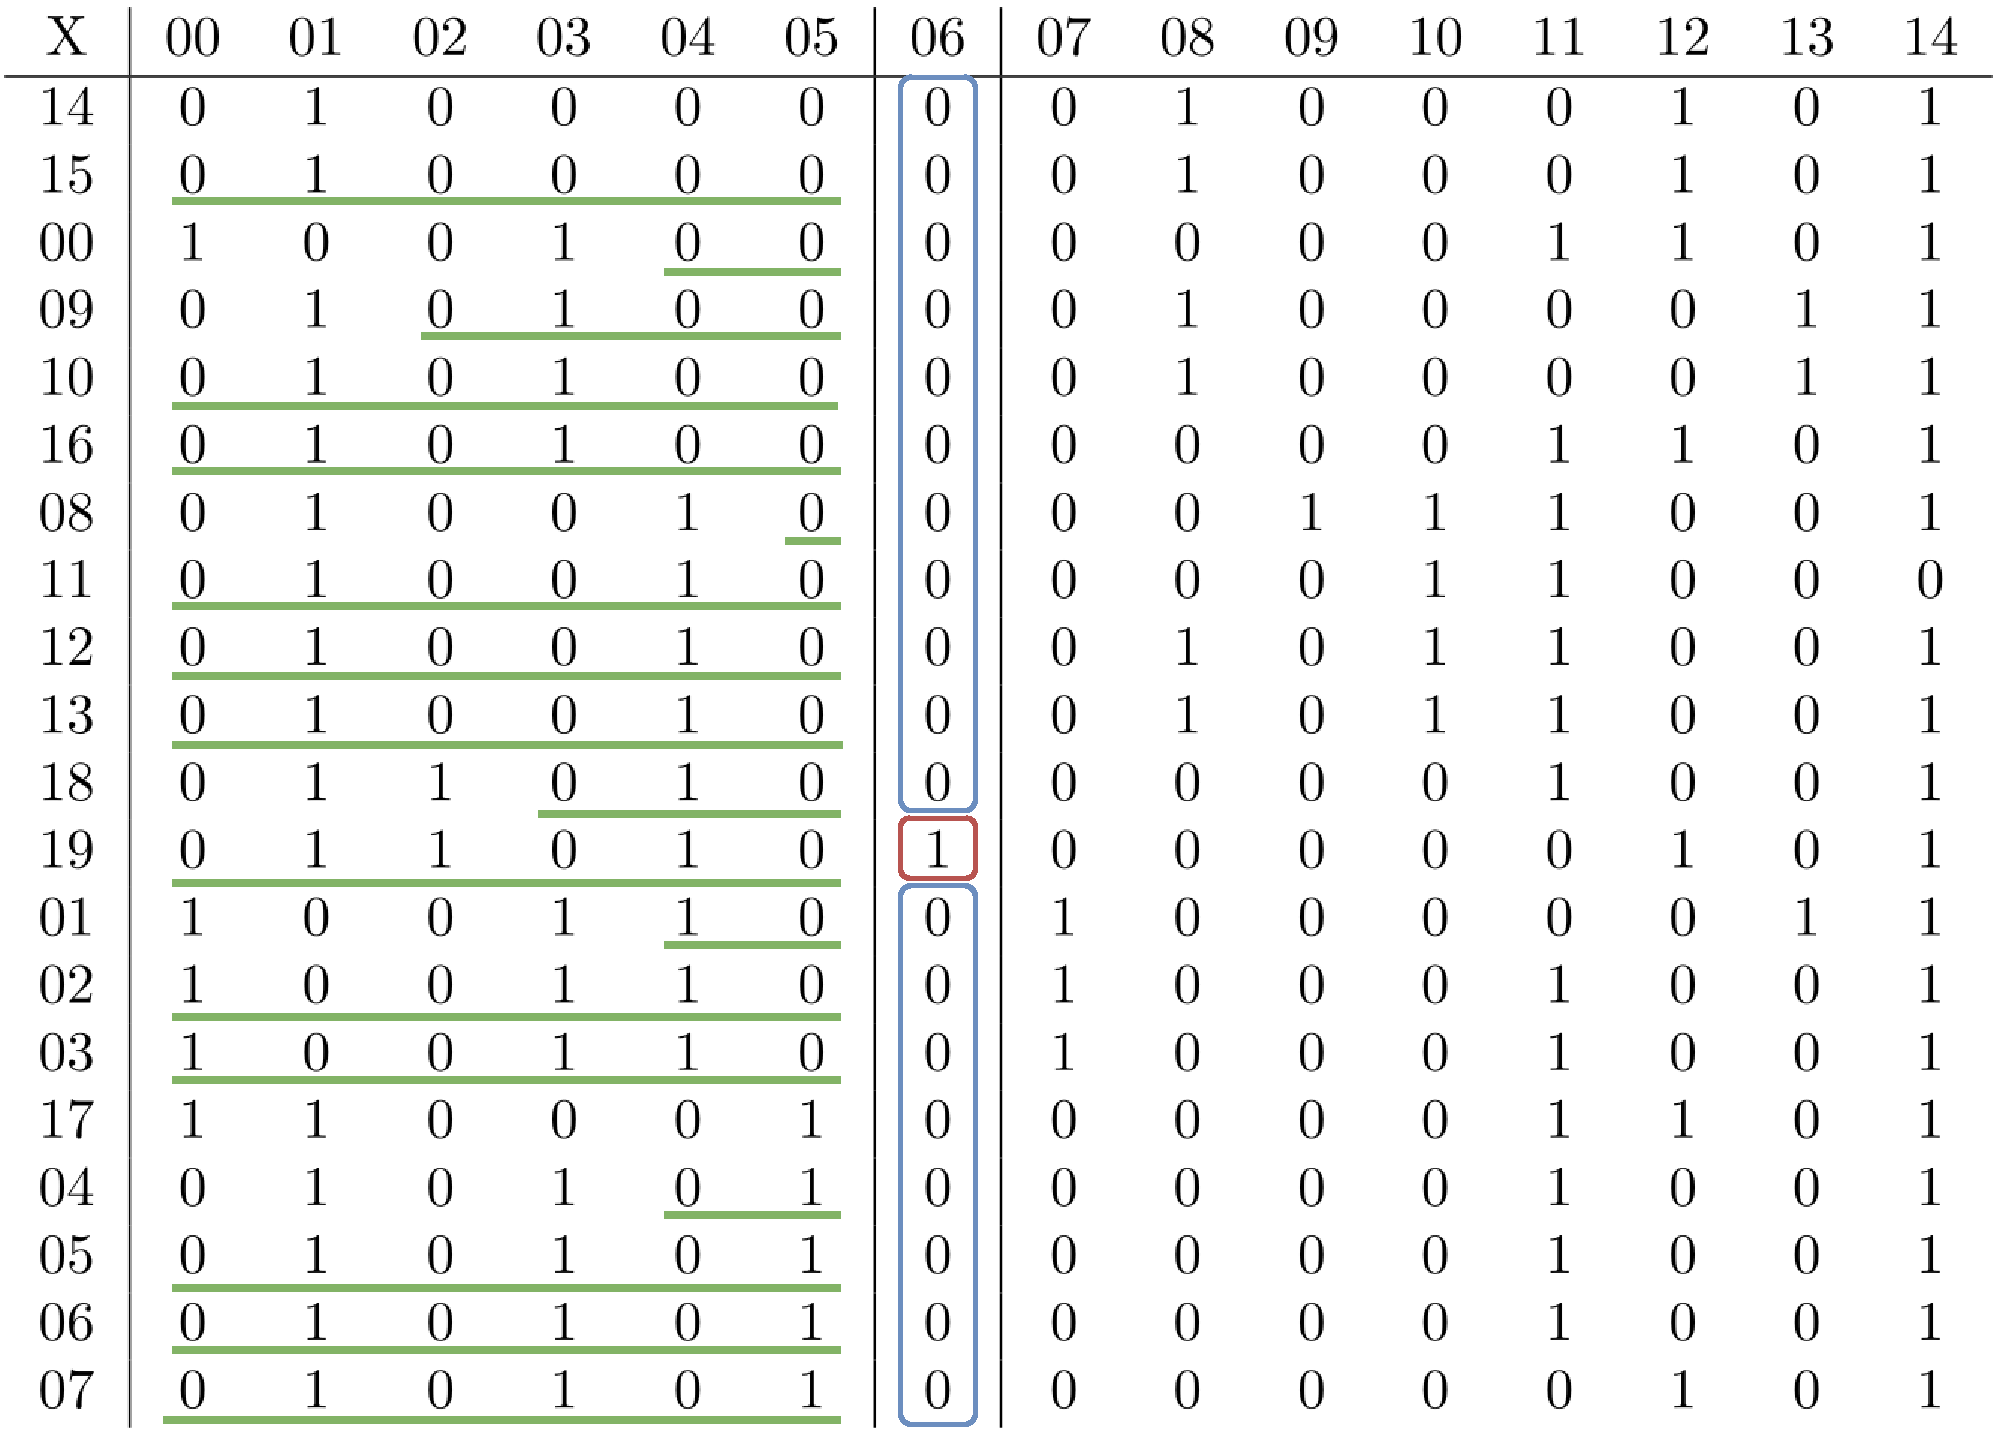
\includegraphics[scale = 0.255]{img/matrix1.pdf}
    \end{figure}
    \vspace{-0.5cm}
    \begin{center}
      {\footnotesize{
        $a_6=[14,15,0,9,10,16,8,11,12,13,18,19,1,2,3,17,4,5,6,7]$\\
        $d_6=[6,0,4,2,0,0,5,0,0,0,3,0,4,0,0,6,4,0,0,0]$
      }}
    \end{center}
  }
  % \only<3>{
  %   \begin{figure}[H]
  %   \centering
  %   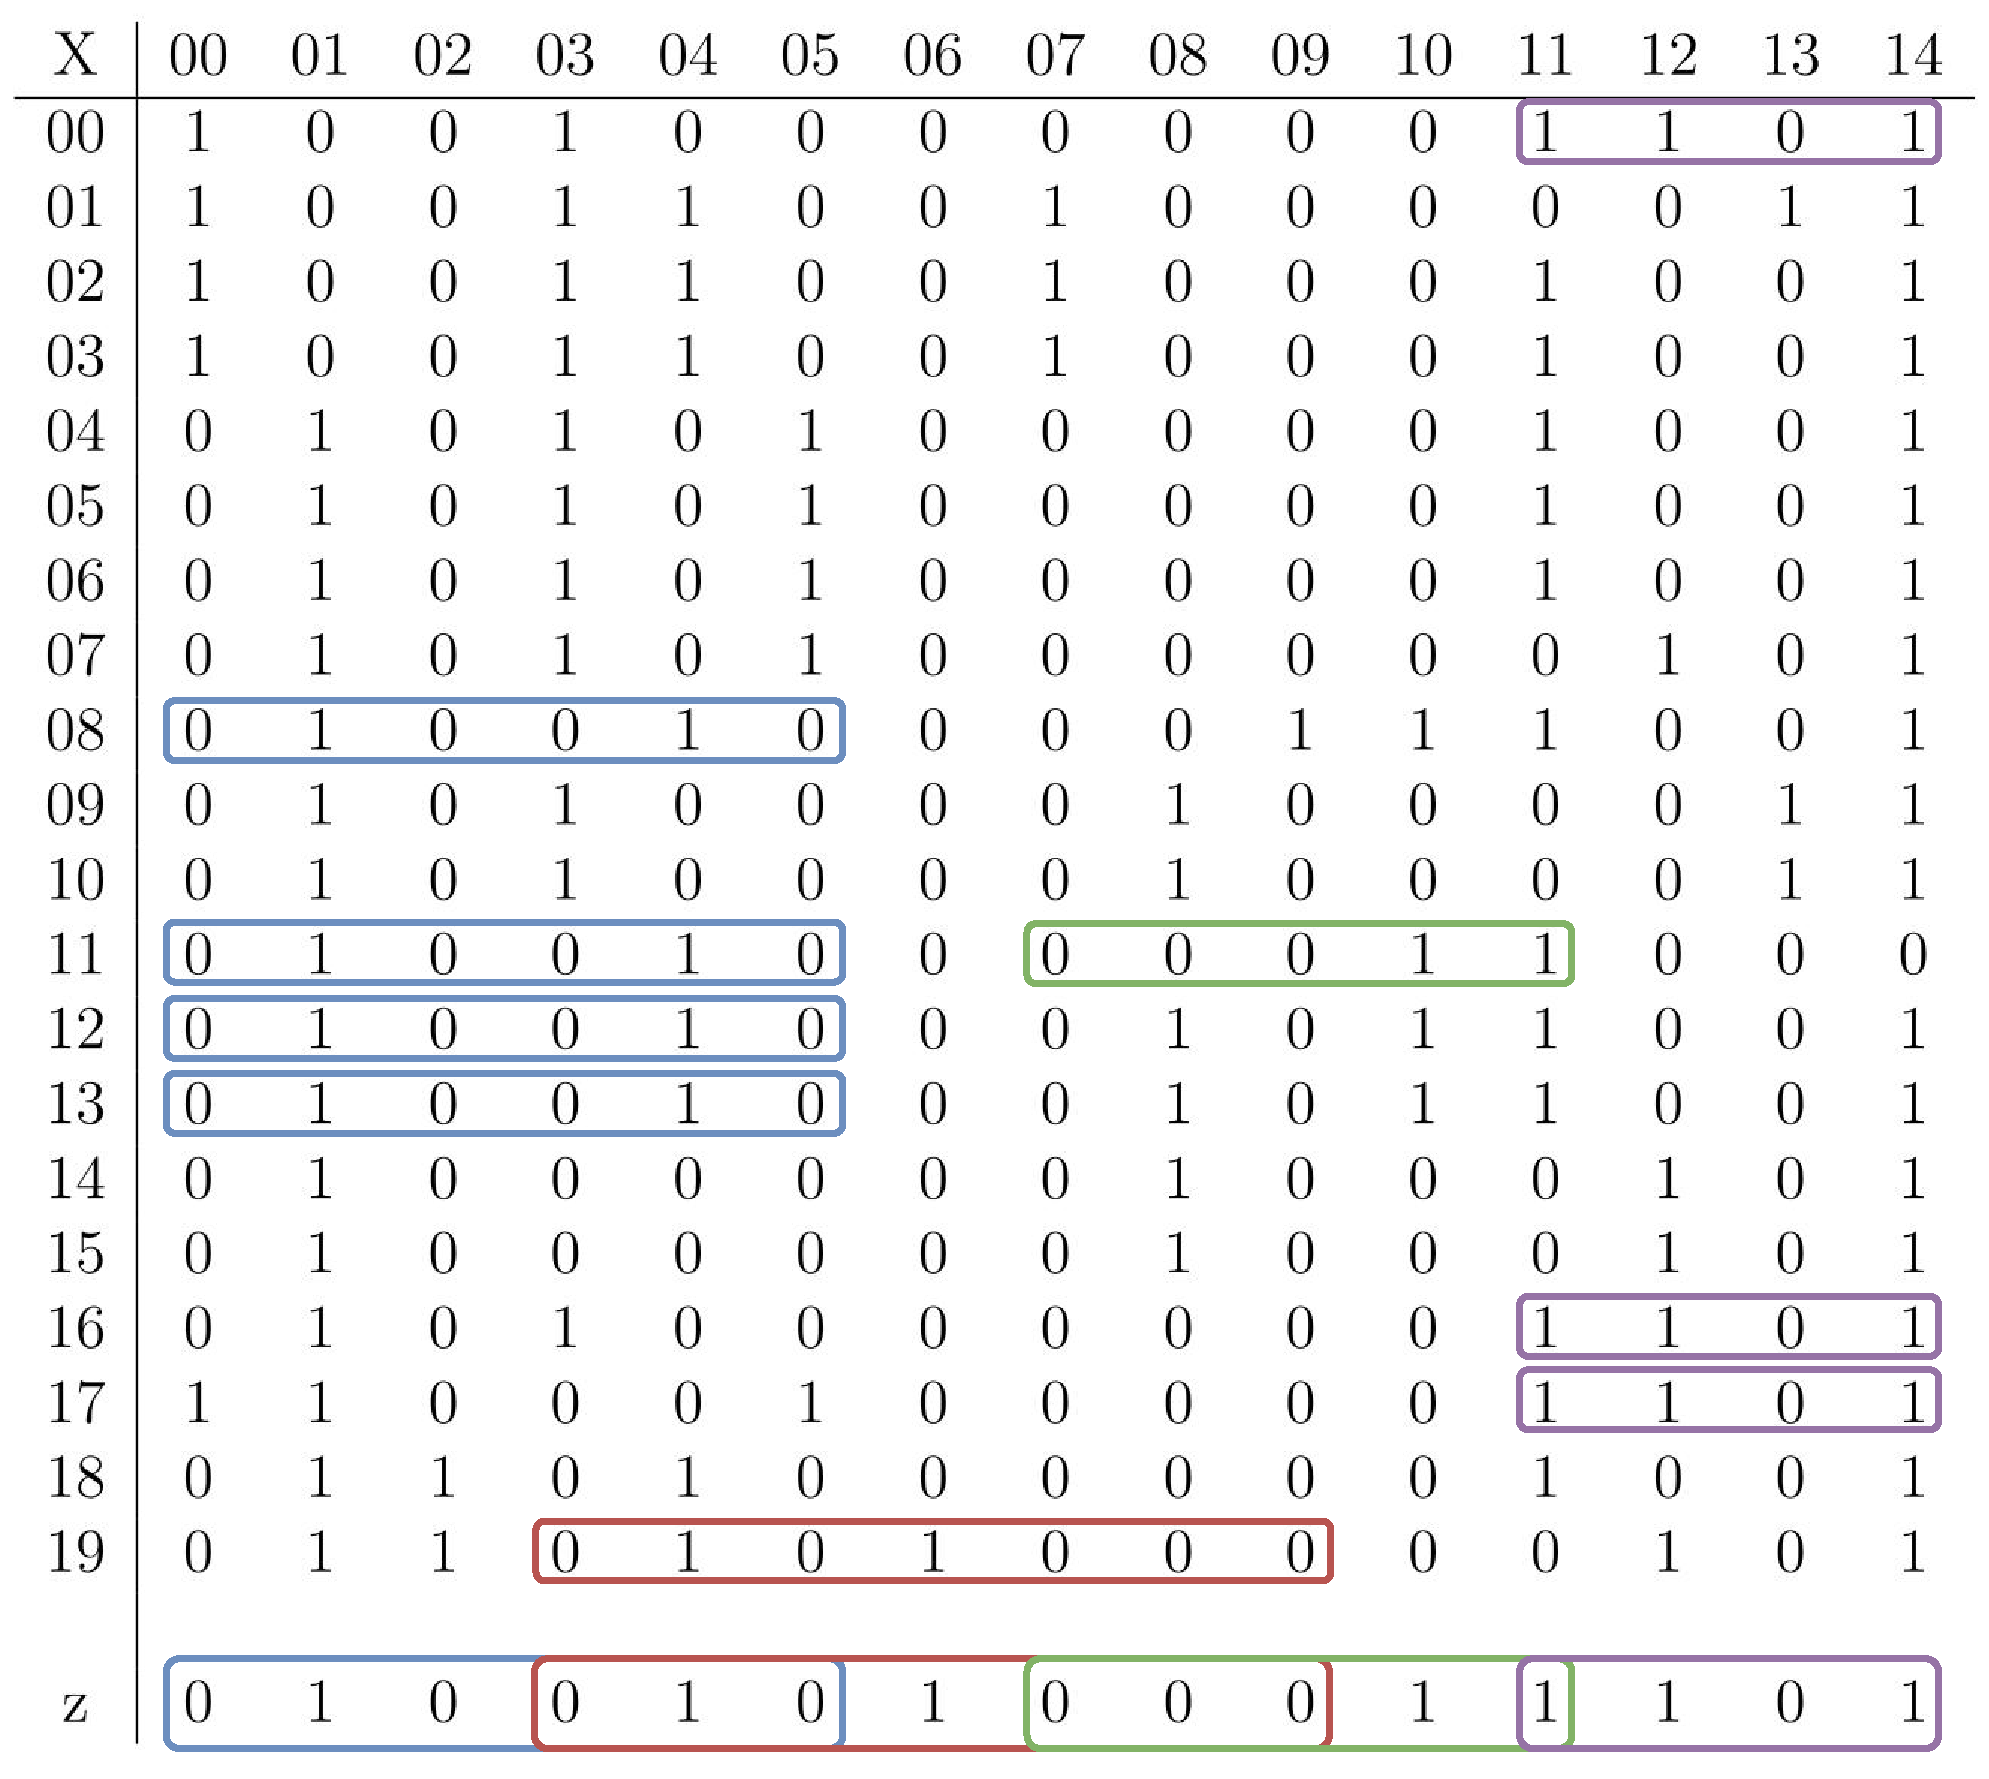
\includegraphics[scale = 0.255]{img/pbwtmatch.pdf}
  % \end{figure}
  % }
\end{frame}
\begin{frame}{Scopo della tesi}
  \begin{block}{}
    Complessità temporale del calcolo degli $\SMEM$ con un algoritmo na\"{i}ve:
    $\mathcal{O}(N^2M)$
  \end{block}
  \begin{block}{}
    Calcolo degli $\SMEM$ con aplotipo esterno per Durbin:
    \begin{itemize}
      \item tempo: $\mathcal{O}(NM)$ + Avg.$\mathcal{O}(N+c)$
      \item spazio: $\mathcal{O}(NM)\implies$ 13NM byte
    \end{itemize}
  \end{block}
  % \begin{block}{}
  %    La $\PBWT$ tendo ad avere simboli uguali in posizioni
  %   consecutive all'interno di ogni sua colonna, a causa del riordinamento e
  %   della natura biologica del dato. 
  % \end{block}
  \begin{alertblock}{}
    Lo scopo di questa tesi è stato quello di creare
    una variante run-length encoded della $\PBWT$ ($\RLPBWT$) che permettesse,
    in modo efficiente dal 
    punto di vista della memoria richiesta, il calcolo degli $\SMEM$ con
    aplotipo esterno. 
  \end{alertblock}
\end{frame}
% \begin{frame}{Alcuni concetti teorici}
%   \begin{block}{}
%     \small{
%     \begin{itemize}
%       \item bitvector, bitvector sparsi e intvector compressi
%       \item straight-line program ($\SLP$) e longest common extension ($\LCE$)
%       query 
%       \item trasformata di Burrows--Wheeler ($\BWT$), (inverse) suffix array
%       ($\IISA$), (permuted) longest common prefix ($\PPLCP$), FM-index,
%       $\LF$-mapping, funzione $\varphi$, maximal exact matches ($\MEM$) e
%       backward-search 
%       \item trasformata di Burrows--Wheeler run-length encoded ($\RLBWT$),
%       r-index, Toehold lemma e matching statistics ($\MS$)
%       \item $\BWT$ posizionale ($\PBWT$) e set-maximal
%       exact match ($\SMEM$)
%     \end{itemize}}
%   \end{block}
%   \begin{block}{}
%     \small{
%     La $\BWT$ ($\PBWT$) tendono ad avere caratteri uguali in posizioni
%     consecutive all'interno della sua sequenza (ogni sua colonna). Si usa il
%     run-length encoding che consiste nel memorizzare le cosiddette run, ovvero
%     sequenze massimali di caratteri uguali, mediante coppie \texttt{(carattere,
%     lunghezza della run)}, ad esempio la stringa \texttt{aaaaaa} sarebbe memorizzata come
%     \texttt{(a,6)}. }
%   \end{block}
% \end{frame}
% \subsection{Bitvector e straight-line program}
% \begin{frame}[fragile]{BV e SLP}
%   \only<1,2>{
%   \begin{block}{BV}
%     \begin{center}
%       \begin{tikzpicture} [nodes in empty cells,
%         nodes={minimum width=0.6cm, minimum height=0.6cm},
%         row sep=-\pgflinewidth, column sep=-\pgflinewidth,ampersand replacement=\&]
%         border/.style={draw}

%         \matrix(vector)[matrix of nodes,
%         row 1/.style={nodes={draw=none, minimum width=0.3cm}},
%         nodes={draw}]
%         {
%         \tiny{0} \& \tiny{1} \& \tiny{2} \& \tiny{3} \& \tiny{4} \& \tiny{5}\&\tiny{6}
%         \& \tiny{7} \& \tiny{8} \& \tiny{9} \& \tiny{10} \& \tiny{11} \& \tiny{12} \&
%         \tiny{13}\\  
%         $\mathbf{1}$ \& $0$ \& $0$ \& $\mathbf{1}$ \& $0$ \& $\mathbf{1}$ \& $0$ \&
%         $\mathbf{1}$ \& $0$ \& $\mathbf{1}$ \& $0$ \& $0$ \& $\mathbf{1}$ \& $0$\\ 
%       };
%       \end{tikzpicture}
%     \end{center}
%     \[\mathtt{rank}(6)=3\quad\quad\mathtt{select}(5) =9\]
%   \end{block}
%   \pause
%   \begin{block}{SLP}
%     \[s=\mbox{GATTAGATACAT}\$\mbox{GATTACATAGAT}\]
%     \[\mbox{S}\to \mbox{ZWAY}\,\$\mbox{ZYAW}\]
%     \vspace{-8mm}
%     \begin{multicols*}{5}
%       \small
%       \begin{itemize}
%         \item $\mbox{Z}\to \mbox{WX}$
%         \item $\mbox{Y}\to \mbox{CV}$
%         \item $\mbox{X}\to \mbox{TA}$
%         \item $\mbox{W}\to \mbox{GV}$
%         \item $\mbox{V}\to \mbox{AT}$
%       \end{itemize}
%     \end{multicols*}
%   \end{block}
% }\only<3>{
%   \begin{block}{SLP}
%     \begin{figure}[H]
%       \centering
%       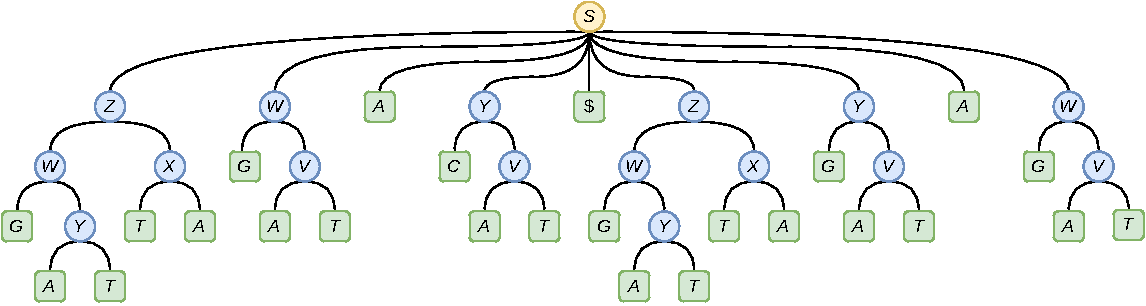
\includegraphics[width=\textwidth]{img/slpgagie.pdf}
%     \end{figure}
%   \end{block}
% }
% \end{frame}
% \subsection{Trasformata di Burrows-Wheeler, suffix array e maximal exact matches} 
%\subsection{Run-length encoded BWT}
% \begin{frame}{RLBWT}
%   \begin{block}{}
%     \begin{table}
%       \scriptsize
%       \begin{tabular}{ P{0.5cm}|P{0.5cm}|P{0.4cm}|P{1.5cm}|P{0.65cm}|P{1.4cm}|P{0.6cm}|P{2.8cm}  }
%         \hline
%         \multicolumn{2}{c|}{Thresholds} & &  &  &  & &  \\
%         \hline
%         {\tt A} & {\tt T}   & $\SA$ & $\SA$ sample  & $\BWT$    & Run heads & $\LCP$ & $\BWM$ \\
%         \hline
%                                         &           & 15    & 15           & {\tt A}   & {\tt A}   & 0 & {\tt \$ATTAGATTACATTA} \\
%         *     &           & 14    & 14           & {\tt T}   & {\tt T}   & 0 & {\tt A\$ATTAGATTACATT} \\
%                                         &            & 9     &              & {\tt T}   &           & 1 & {\tt ACATTA\$ATTAGATT} \\
%                                         &            & 4     &              & {\tt T}   &           & 1 & {\tt AGATTACATTA\$ATT} \\
%                                         &           & 11    & 11            & {\tt C}   & {\tt C}   & 1 & {\tt ATTA\$ATTAGATTAC} \\
%                                         &           & 6     & 6             & {\tt G}   & {\tt G}   & 4 & {\tt ATTACATTA\$ATTAG} \\
%                                         &           & 1     & 1             & {\tt \$}  & {\tt \$}  & 4 & {\tt ATTAGATTACATTA\$} \\
%                                         &    *       & 10    & 10            & {\tt A}   & {\tt A}   & 0 & {\tt CATTA\$ATTAGATTA} \\
%                                         &           & 5     &               & {\tt A}   &          & 0 & {\tt GATTACATTA\$ATTA} \\
%         *     &           & 13    & 13            & {\tt T}   & {\tt T}   & 0 & {\tt TA\$ATTAGATTACAT} \\
%                                         &           & 8     &               & {\tt T}   &           & 2 & {\tt TACATTA\$ATTAGAT} \\
%                                         &           & 3     &               & {\tt T}   &           & 2 & {\tt TAGATTACATTA\$AT} \\
%                                         &           & 12    & 12            & {\tt A}   & {\tt A}   & 1 & {\tt TTA\$ATTAGATTACA} \\
%                                         &           & 7     &               & {\tt A}  &           & 3 & {\tt TTACATTA\$ATTAGA} \\
%                                         &           & 2     &               & {\tt A}  &           & 3 & {\tt TTAGATTACATTA\$A} \\  
%         \hline
%       \end{tabular}
%     \end{table}
%   \end{block}
  
% \end{frame}
%\subsection{Matching statistics e maximal exact matches} 
% \begin{frame}{MS e MEM}
%   \begin{block}{MS}
%     \footnotesize
%     Dato un testo $T$, con $|T|=n$, e un pattern $P$, con $|P|=m$, si
%     definisce \textbf{matching statistics} di $P$ su $T$ un array $MS$ di
%     coppie $(pos, len)$, lungo quanto il pattern, tale che:
%     \begin{itemize}
%       \item $T[MS[i].pos,MS[i].pos+MS[i].len-1]=P[i,i+MS[i].len-1]$, quindi si
%       ha un match tra $P$ e $T$ lungo $MS[i].len$ a partire da $MS[i].pos$ in
%       $T$ e da $i$ in $P$
%       \item $P[i,i+MS[i].len]$ non occorre in $T$, quindi il match non è
%       ulteriormente estendibile 
%     \end{itemize}
%   \end{block}
%   \pause
%   \begin{block}{MEM}
%     \footnotesize
%     Dato un testo $T$, con $|T|=n$, e un pattern $P$, con $|P|=m$, si definisce
%     una sottostringa $P[i,i+l-1]$, di lunghezza $l$, \textbf{MEM} di $P$ in $T$
%     se:
%     \begin{itemize}
%       \item $P[i,i+l-1]$ è una sottostringa di $T$
%       \item $P[i-1,i+l-1]$ non è una sottostringa di $T$ (non si può estendere a
%       sinistra) e $P[i,i+l]$ non è una sottostringa di $T$ (non si può estendere a
%       destra) 
%     \end{itemize}
%     Un MEM si può calcolare dalle MS:
%     \[MS[i].len=l\land MS[i-1].len\leq MS[i].len\]
%   \end{block}
% \end{frame}
% \subsection{Run-length BWT, MONI e PHONI}
% \begin{frame}{MONI e PHONI}
%   \begin{block}{MONI}
%     \small
%     Rossi et al., nel 2021, sfruttarono le conoscenze relative
%     alla $\RLBWT$ e all'r-index 
%     per ideare \textbf{MONI}. In questa soluzione si ha la costruzione, in due
%     sweep, tramite l'uso delle threshold (\textit{algoritmo di
%       Bannai}), dell'array delle matching statistics, da cui si computano i
%     maximal exact match. 
%   \end{block}
%   \begin{alertblock}{}
%     \footnotesize{\textit{\textbf{Rossi et al.:}
%         MONI: A pangenomic index for finding maximal exact matches, 2021}}
%   \end{alertblock}
%   % \pause
%   % \begin{block}{LCE}
%   %   \small
%   %   Dato un testo $T$, tale che $|T|=n$, il risultato della \textbf{LCE query}
%   %   tra 
%   %   due posizioni $i$ e $j$, tali che $0\leq i,j<n$, corrisponde al più lungo
%   %   prefisso comune tra le sotto-stringhe che hanno come indice di partenza
%   %   $i$ e 
%   %   $j$, avendo quindi il più lungo prefisso comune tra $T[i,n-1]$ e
%   %   $T[j,n-1]$. 
%   % \end{block}
%   \begin{block}{PHONI}
%     \small
%     Nel 2021, Boucher, Gagie, Rossi et al. proposero un ulteriore miglioramento di
%     quanto fatto in MONI, con \textbf{PHONI}, usando le
%     $\LCE$ query 
%     al posto delle threshold, ottenendo un algoritmo ``online''.
%   \end{block}
%   \begin{alertblock}{}
%     \footnotesize{\textit{\textbf{Boucher et al.:}
%         PHONI: Streamed matching statistics with multi-genome references, 2021}}
%   \end{alertblock}
% \end{frame}
% \subsection{Trasformata di Burrows-Wheeler posizionale}
% \begin{frame}{PBWT}
%   % \only<1,2>{
%   % \begin{block}{Prefix array}
%   %   Dato un aplotipo $i$, appartenente al pannello $X$, e un indice di colonna
%   %   $k$, si definisce il \textbf{prefix array} $a_k$ come una permutazione
%   %   degli indici $0,\ldots, M-1$ tale che $a_k[i]=j$ sse $x_j$ è l'$i$-esimo
%   %   aplotipo di $X$ nell'ordinamento inverso dei prefissi ottenuto alla
%   %   colonna $k$. Quindi $a_k[i]=m$, con $m<M$, altro non è che l'indice della
%   %   sequenza $x_m$ del pannello $X$ da cui deriva il prefisso $i$-esimo
%   %   nell'ordine inverso in colonna $k$.
%   % \end{block}
%   % \pause
%   % \begin{block}{Divergence array}
%   %   Si definisce \textbf{divergence array} l'array $d_k$ tale che $d_k[i]$ è
%   %   l'indice colonna iniziale del match massimale a sinistra terminante in $k$
%   %   tra 
%   %   l'$i$-esimo aplotipo e il suo precedente nell'ordinamento ottenuto alla
%   %   colonna $k$-esima. Formalmente, dato $i>0$, si definisce 
%   %   $d_k[i]$ come il più piccolo $j$ tale che $y_i^k[j,k)=y_{i-1}^k[j,k)$.
%   %   Ne segue che $y_i^k[k-1]\neq y_{i-1}^k[k-1] \implies d_k[i]=k$ (per
%   %   definizione $d_k[0]=k$).
%   % \end{block}
%   % }\only<3>{
%   \begin{figure}[H]
%     \centering
%     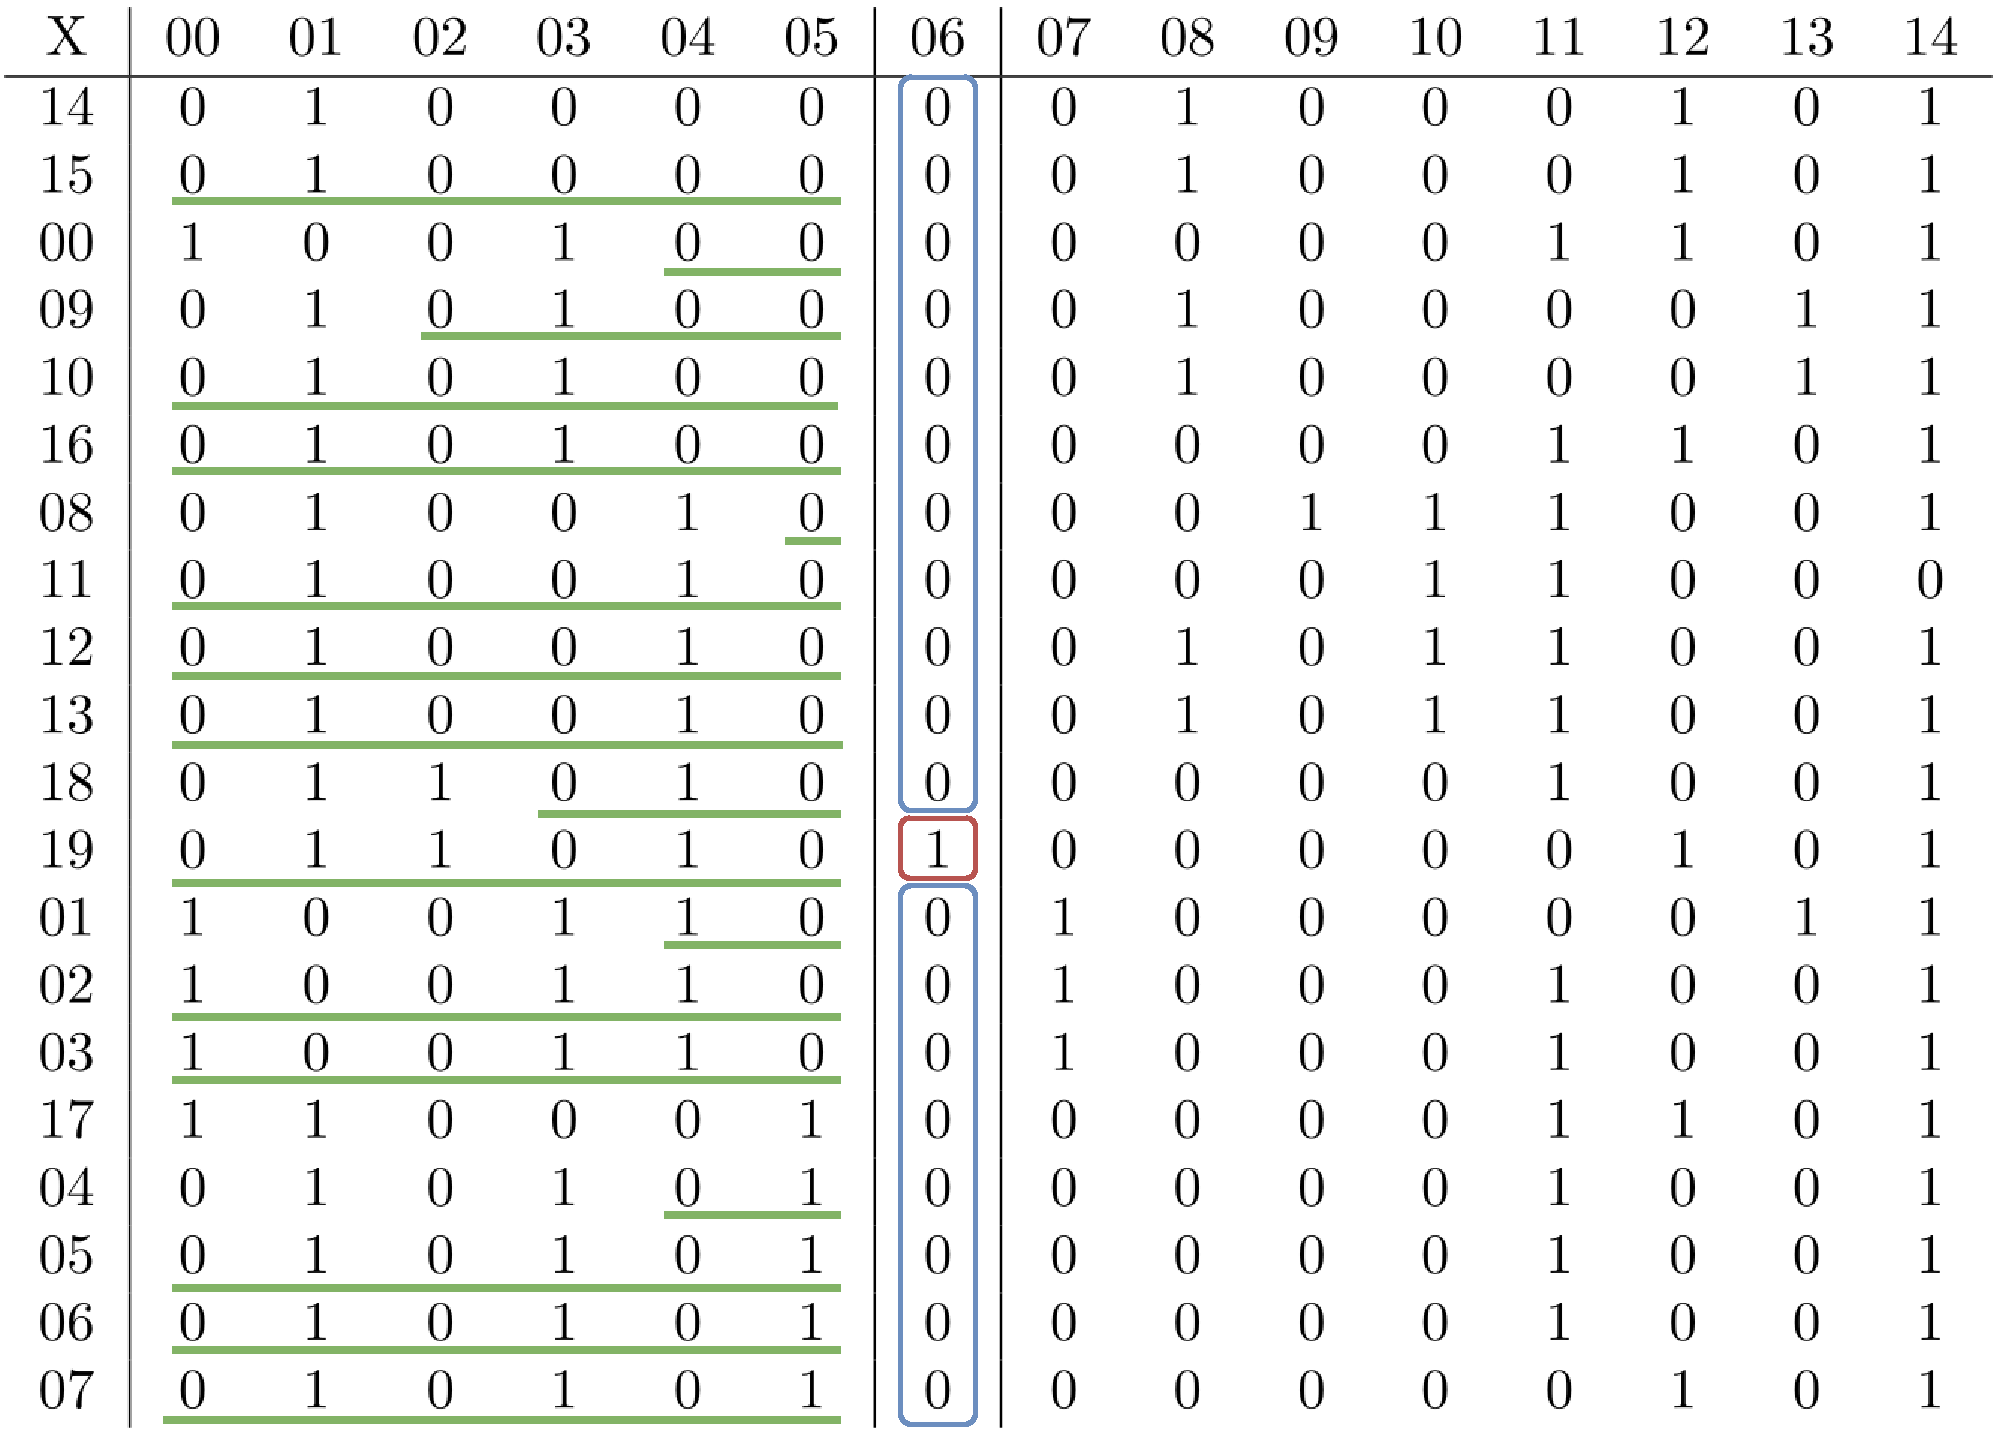
\includegraphics[scale = 0.205]{img/matrix1.pdf}
%   \end{figure}
%   \vspace{-0.2cm}
%   {\scriptsize{
%       $a_6=[14,15,0,9,10,16,8,11,12,13,18,19,1,2,3,17,4,5,6,7]$\\
%       $d_6=[6,0,4,2,0,0,5,0,0,0,3,0,4,0,0,6,4,0,0,0]$
%     }}
%   % {\footnotesize{\[a_6=[14,15,0,9,10,16,8,11,12,13,18,19,1,2,3,17,4,5,6,7]\]
%   % \[d_6=[6,0,4,2,0,0,5,0,0,0,3,0,4,0,0,6,4,0,0,0]\]}}
%   \vspace{-0.1cm}
%   \begin{alertblock}{}
%     \footnotesize{\textit{\textbf{Durbin:}
%         Efficient haplotype matching and storage using the positional
%         Burrows--Wheeler transform (PBWT), 2014}}
%   \end{alertblock}
% \end{frame}
% \subsection{Set-maximal exact match con la PBWT}
% \begin{frame}{Set-maximal exact match}
%   \begin{block}{}
%     \small{Calcolo $\SMEM$ via \textbf{algoritmo 5 di
%         Durbin} in tempo $\mathcal{O}(NM)$ + Avg.$\mathcal{O}(N+c)$,
%       richiedendo 13NM byte}
%   \end{block}
%   \begin{figure}[H]
%     \centering
%     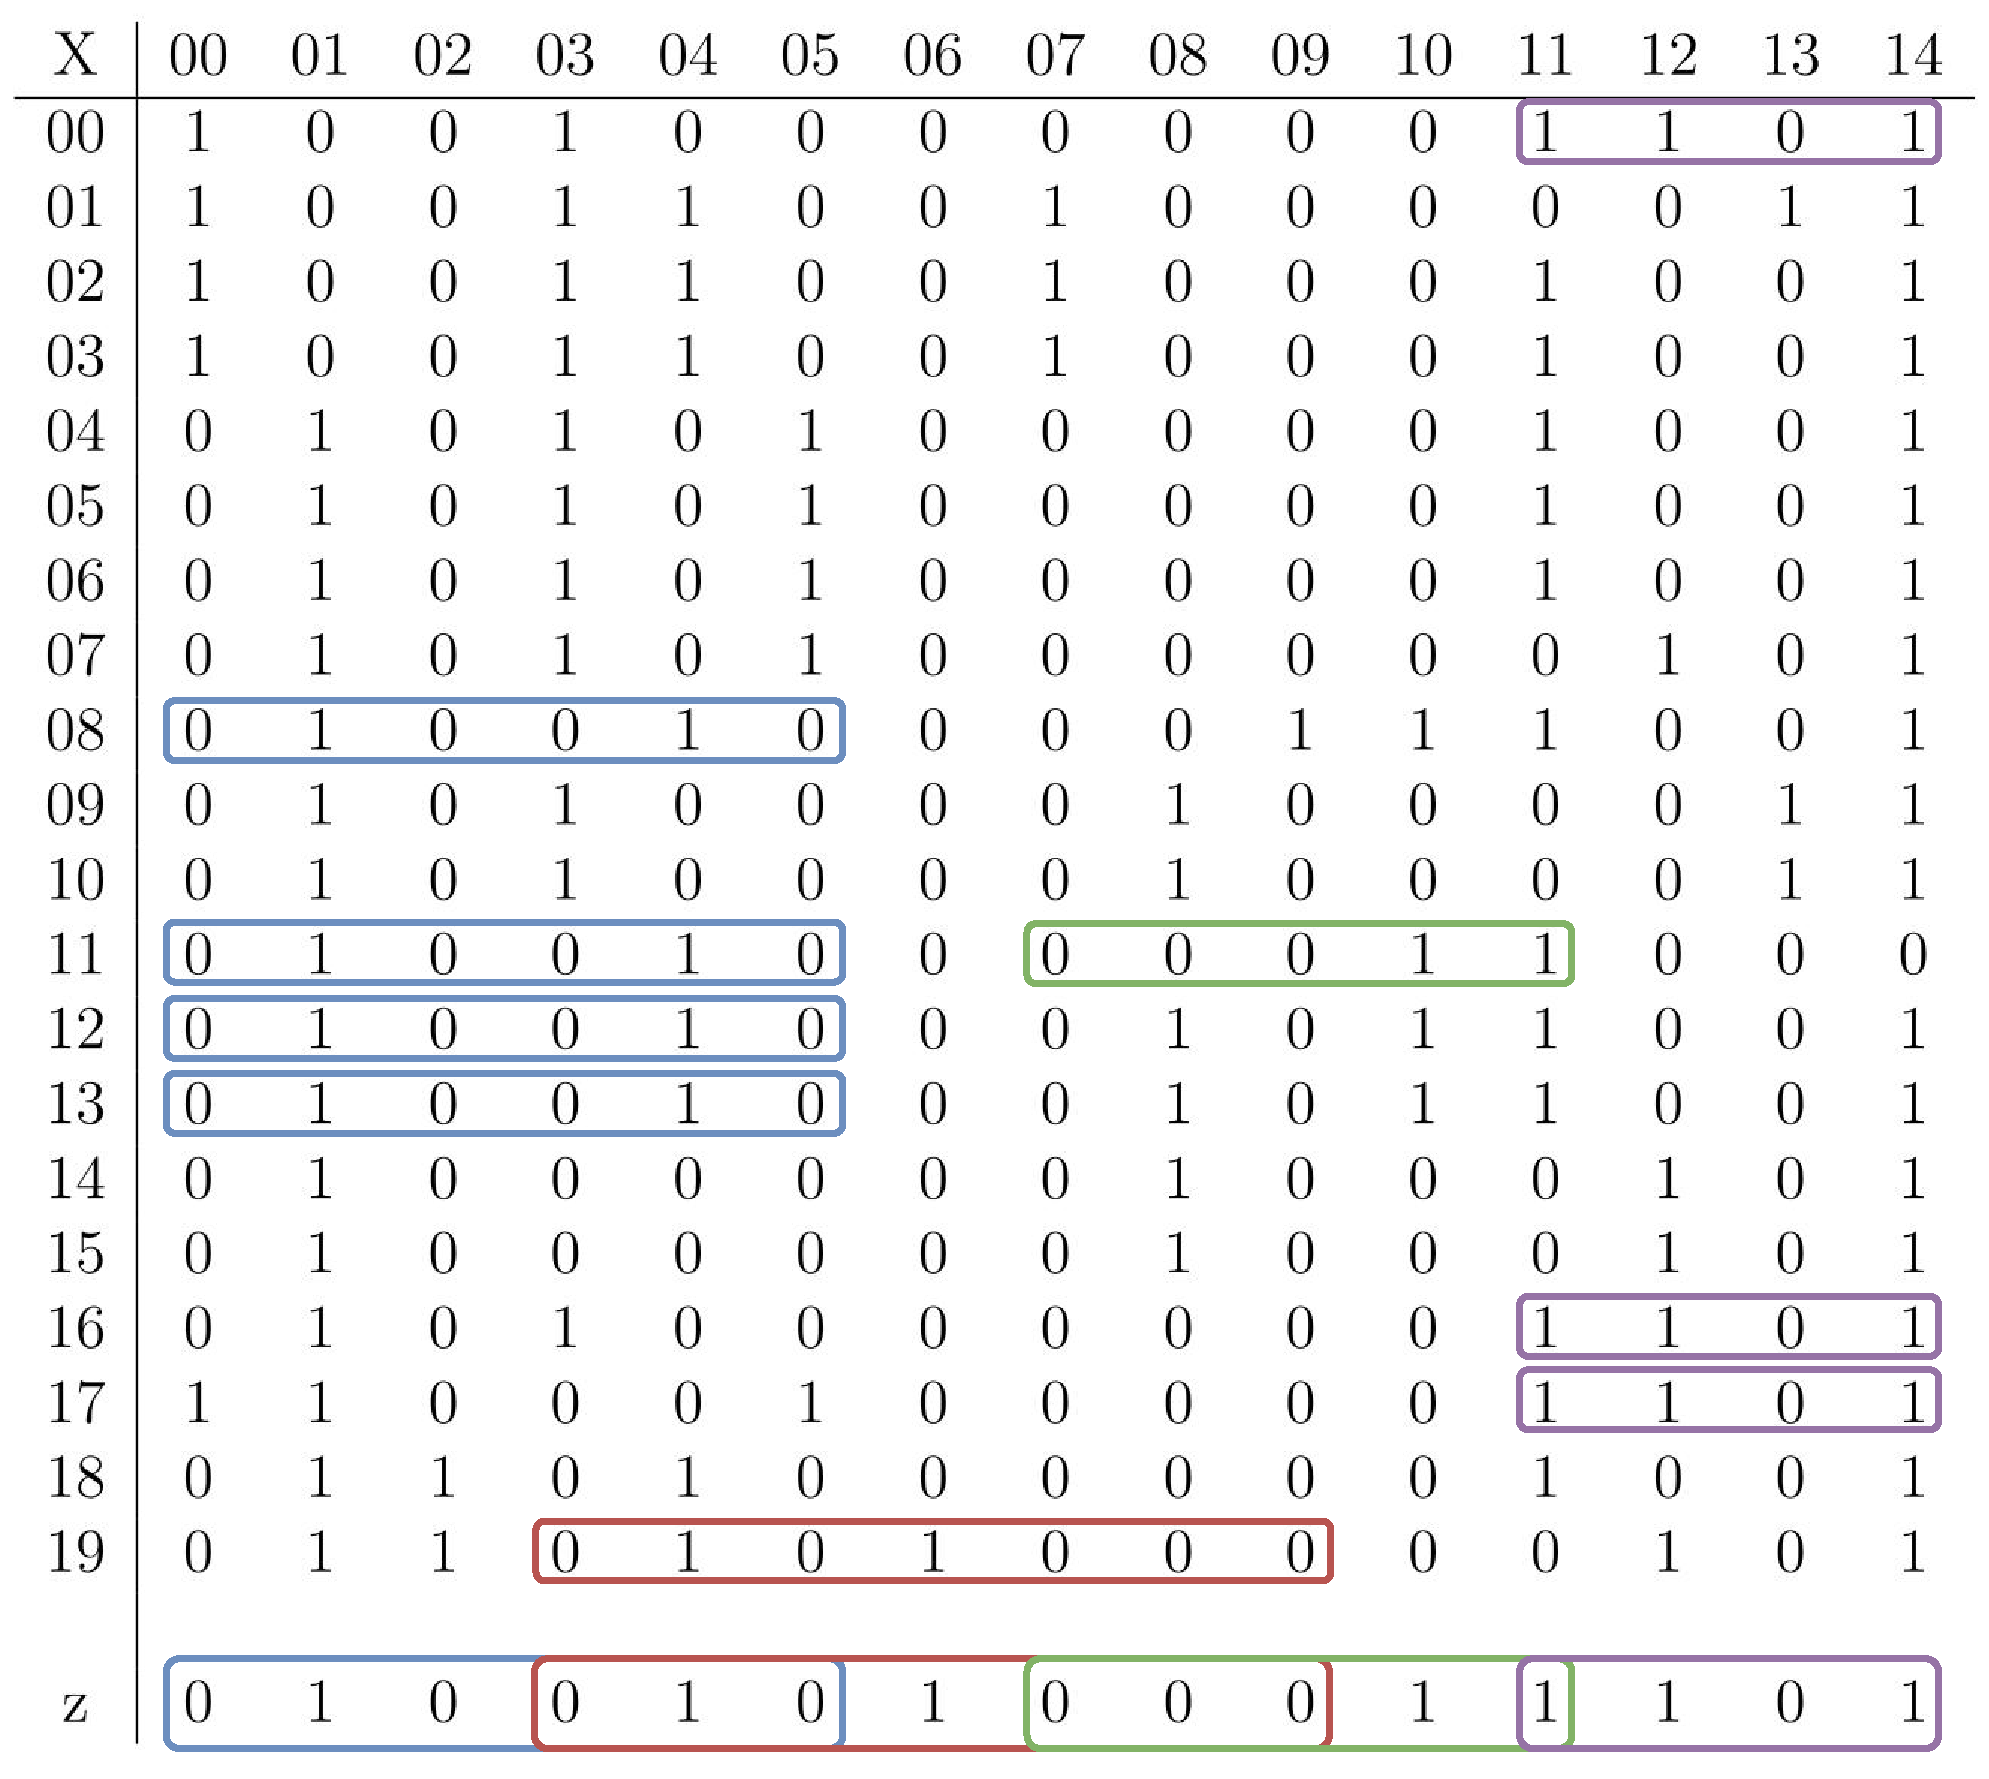
\includegraphics[scale = 0.205]{img/pbwtmatch.pdf}
%   \end{figure}
  
%   % Dato un pannello $X$, con $M$ aplotipi/righe e $N$ siti/colonne, e un
%   % aplotipo 
%   % query $z$, tale che $|z|=N$, si definisce un \textbf{Set-Maximal Exact
%   % Match}  
%   % ($\SMEM$), iniziante in colonna $e_k$ e terminante il colonna
%   % $k$, tra 
%   % la query $z$ e le righe del pannello indicizzate dai valori compresi
%   % nell'intervallo $[f_k,g_k)$ in $a_k$ sse:
%   % \[z[e_k,k)=y_i^k[e_k,k)\land z[e_k-1]\neq y_i^k[e_k-1], \forall\, i\mbox{
%   %   t.c. }f_k\leq i < g_k\]
%   % Si noti che $g_k=M$ sse $y_{M-1}^k$ appartiene alle righe per le quali si ha
%   % tale $\SMEM$.
% \end{frame}
\section{Contributo della tesi}
\subsection{Componenti per la RLPBWT}
\begin{frame}{Le componenti}
  \begin{block}{Componenti innovative derivate dallo studio della $\RLBWT$ in
      ottica $\PBWT$} 
    \begin{itemize}
      \item mapping tra una colonna e la successiva nella
      $\PBWT$ e threshold:
      \begin{itemize}
        \item bitvector sparsi, con $\rank$ in
        $\mathcal{O}\left(\log\left(\frac{M}{\rho}\right)\right)$:
        \underline{\texttt{MAP-BV}} e \underline{\texttt{THR-BV}}
        \item intvector compressi, con $\rank$ in
        $\mathcal{O}\left(\log\left(\rho\right)\right)$:
        \underline{\texttt{MAP-INT}} e  \underline{\texttt{THR-INT}}
      \end{itemize}
      \item random access:
      \begin{itemize}
        \item bitvector, in $\mathcal{O}(1)$: \underline{\texttt{RA-BV}}
        \item $\SLP$, in $\mathcal{O} (\log(NM))$: \underline{\texttt{RA-SLP}}
      \end{itemize}
      \item $\LCE$ query con $\SLP$, in $\mathcal{O} (\log(NM))$:
      \underline{\texttt{LCE}}
      \item prefix array sample: \underline{\texttt{PERM}}  
      \item struttura per le funzioni $\varphi$ e $\varphi^{-1}$:
      \underline{\texttt{PHI}} 
      %\item reverse longest common prefix: \underline{\texttt{RLCP}}
    \end{itemize}
  \end{block}
\end{frame}
\begin{frame}{Qualche confronto in spazio}
  \begin{figure}[H]
    \centering
    \hspace{-0.2cm}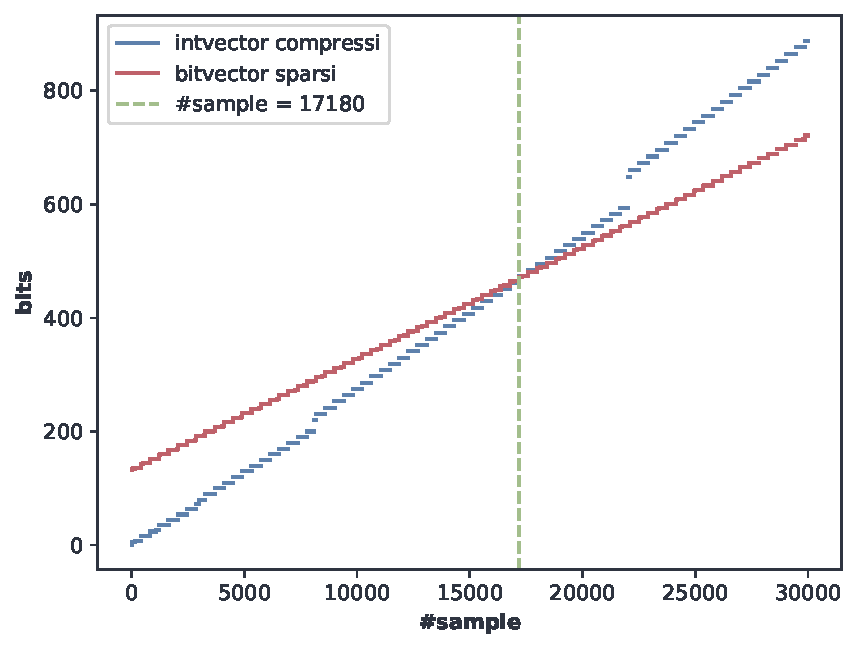
\includegraphics[width=0.8\textwidth]{img/bv_vs_iv.pdf}
    %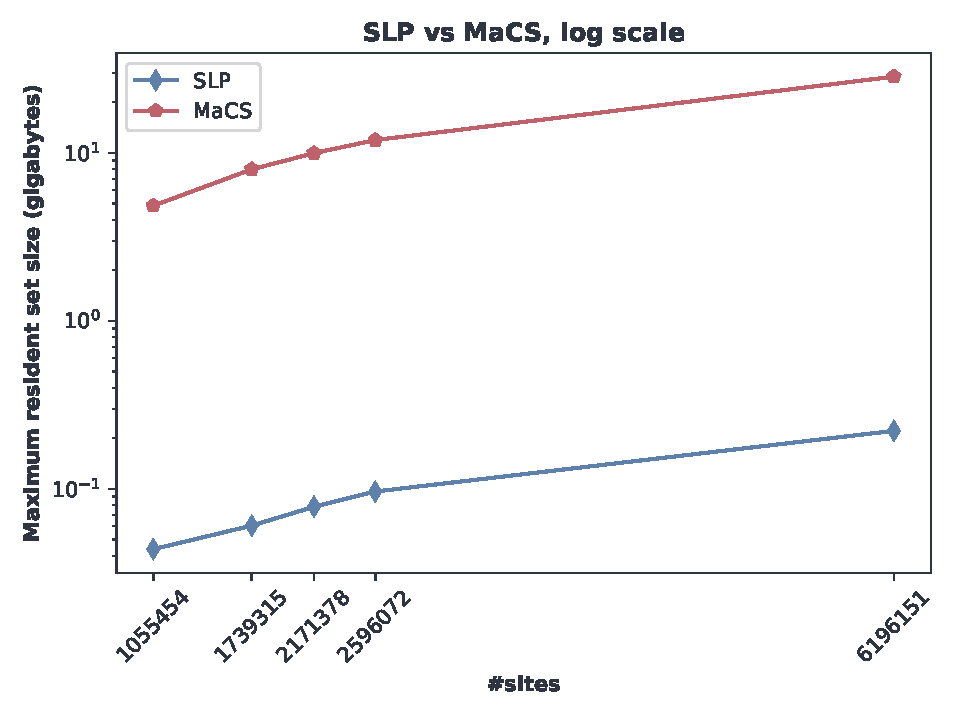
\includegraphics[width=0.49\textwidth]{img/slp_vs_macs_log.pdf}

  \end{figure}
\end{frame}
\subsection{Strutture dati per la RLPBWT e calcolo degli SMEM}
% \begin{frame}{Le strutture dati}
%   \begin{block}{Strutture per il calcolo degli $\SMEM$ tramite $\RLCP$, non in
%       grado di calcolare quali righe presentino uno $\SMEM$ ma solo quante.}
%     \begin{itemize}
%       \item \texttt{MAP-BV + RLCP}
%       \item \texttt{MAP-INT + RLCP}
%     \end{itemize}
%   \end{block}
%   \begin{block}{Strutture per il calcolo degli $\SMEM$ tramite $\MS$, in grado
%       di calcolare tutte le righe che presentano uno $\SMEM$.}
%     \begin{itemize}
%       \item \texttt{MAP-BV + THR-BV + RA-BV + PERM + PHI}
%       \item \texttt{MAP-BV + THR-BV + RA-SLP + PERM + PHI}
%       \item \texttt{MAP-INT + THR-INT + RA-BV + PERM + PHI}
%       \item \texttt{MAP-INT + THR-INT + RA-SLP + PERM + PHI}
%       \item \texttt{MAP-BV + LCE + PERM + PHI}
%       \item \texttt{MAP-INT + LCE + PERM + PHI}
%     \end{itemize}
%   \end{block}
% \end{frame}
\begin{frame}{Calcolo degli $\SMEM$}
  \begin{block}{Matching statistics per la $\PBWT$}
    {\small{
        Dato un pannello $X=\{x_0,\ldots,x_{M-1}\}$, $x_i=N$,
        e un aplotipo esterno/pattern $z$, tale che $|z|=N$, si definisce
        \textbf{matching
        statistic}s di $z$ su $X$ un array $\MS$ di coppie $(\row,\len)$, 
        $|\MS|=N$, tale che:   
        \begin{itemize}
          \item $x_{\MS[i].\row}[i-\MS[i].\len+1,i]=z[i-\MS[i].\len+1,i]$, ovvero si
          ha che 
          l'aplotipo query ha un match, lungo $\MS[i].\len$, terminante in colonna
          $i$, con la riga 
          $\MS[i].\row$-esima del pannello
          \item $z[i-\MS[i].\len,i]$ non è un suffisso terminante in colonna $i$
          di un qualsiasi sottoinsieme di righe di $X$
        \end{itemize}
      }}
  \end{block}
  \pause
  \begin{block}{$\SMEM$ da $\MS$}
    {\small{
        Dato un array di matching statistics $\MS$ si ha che $z[i-l+1,i]$
        presenta uno $\SMEM$ di lunghezza $l$ con la riga $\MS[i].\row$-esima
        del 
        pannello $X$ sse: 
        $\MS[i].\len=l\land(i=N-1\lor \MS[i].\len\geq \MS[i+1].\len)$
      }}
  \end{block}
\end{frame}
\begin{frame}{Componenti e strutture dati, una panoramica}
  \begin{figure}[H]
    \centering
    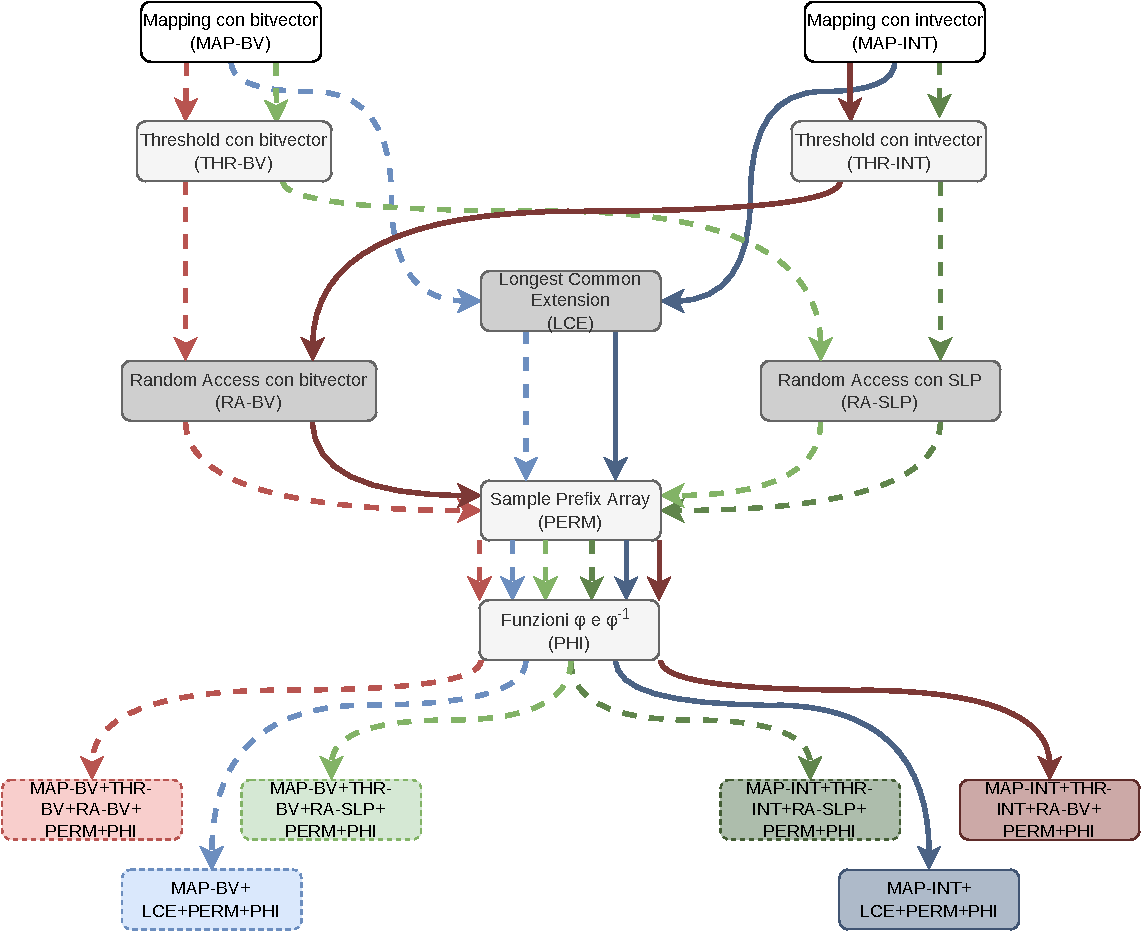
\includegraphics[width=0.8\textwidth]{img/ds2.pdf}
  \end{figure}
\end{frame}
\begin{frame}{Matching statistics}
  \vspace{-0.35cm}
 \begin{figure}[H]
    \centering
    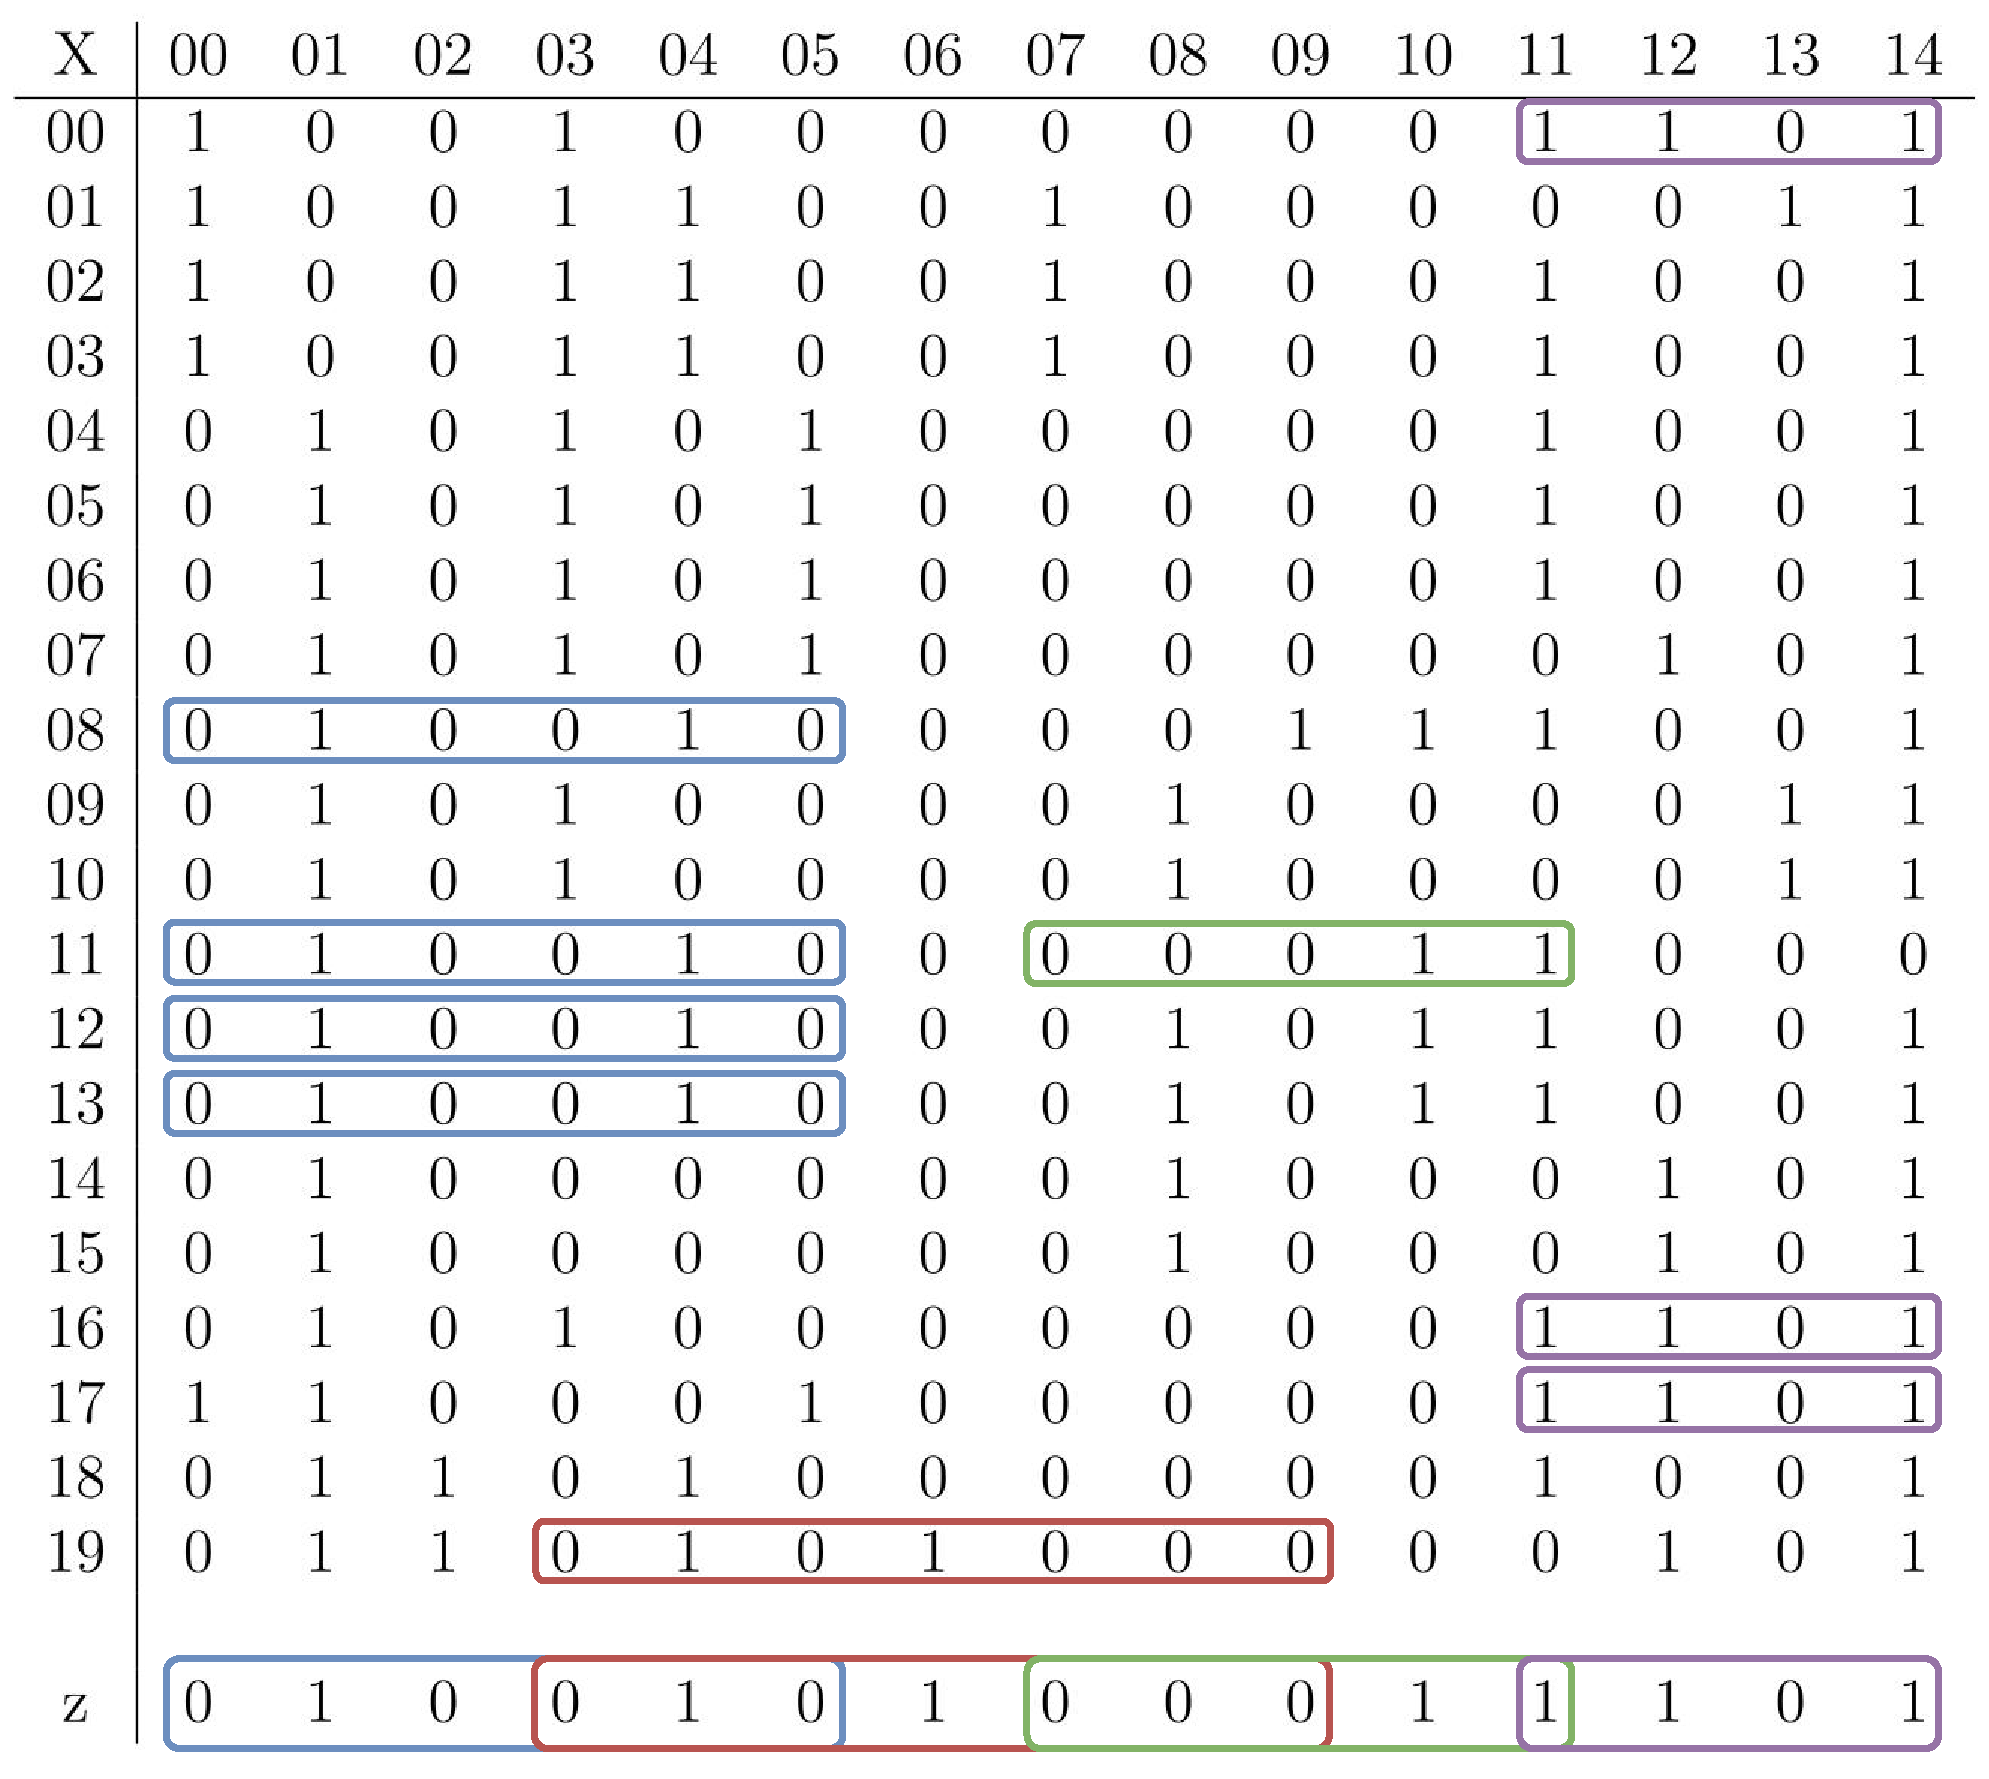
\includegraphics[scale = 0.205]{img/pbwtmatch.pdf}
  \end{figure}
  \vspace{-0.5cm}
  \begin{table}[H]
    \scriptsize
    \centering
    \begin{tabular}{c|ccccccccccccccc}
      $k$ & 00 & 01 & 02 & 03 & 04 &  {\color{nordcyan}05} & 06 & 07 & 08
      &  {\color{nordred}09} & 10 &  {\color{nordgreen}11} & 12 & 13
      &  {\color{nordpurple}14} \\
      \hline
      $\row$ & 19 & 19 & 16 & 15 & 13 &  {\color{nordcyan}13} & 19 & 19 & 19
      &  {\color{nordred}19} & 11 &  {\color{nordgreen}11} & 17 & 17
      &  {\color{nordpurple}17} \\
      $\len$ & 1 & 2 & 3 & 4 & 5 & {\color{nordcyan}6} & 4 & 5 & 6
      & {\color{nordred}7} & 4 & {\color{nordgreen}5} & 2 & 3
      & {\color{nordpurple}4}\\
    \end{tabular}
  \end{table}
\end{frame}
\begin{frame}{Struttura per le funzioni $\varphi$ e $\varphi^{-1}$}
  \begin{figure}[H]
    \centering
    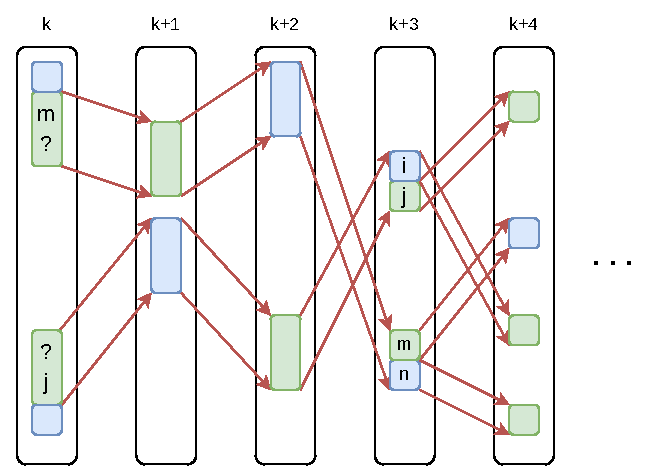
\includegraphics[scale = 0.8]{img/phi.pdf}   
  \end{figure}
  % {\footnotesize{\[\varPhi_j=[0,0,0,1,0, \ldots],\quad
  %       \varPhi^{-1}_m=[0,0,0,1,0,\ldots],\quad
  %       \varPhi_{supp}=[i,\ldots],\quad
  %       \varPhi^{-1}_{supp}=[n,\ldots]\]}}
  % \[\varPhi_{supp}^j[\rank^\varphi_j(0)]=\varPhi_{supp}^j[0]=i,\quad
  %   \varPhi^{-1\,\,m}_{supp}[\rank^{\varphi^{-1}}_m(0)]=\varPhi^{-1\,\,m}_{supp}[0]=n\]
  
\end{frame}
\section{Risultati sperimentali}
\subsection{Setup sperimentale}
\begin{frame}{Sperimentazione e dati}
   \begin{block}{Implementazione e sperimentazione}
    \small
    La sperimentazione, orchestrata tramite \texttt{snakemake}, è stata
    effettuata su una macchina con processore 
    Intel Xeon E5-2640 V4 ($2,40$GHz), $756$GB di RAM, $768$GB di swap e
    sistema operativo Ubuntu 20.04.4 LTS.\\
    Si sono confrontate l'implementazione in \Cplusplus $\,\,$della $\RLPBWT$ e
    l'implementazione in C ufficiale della $\PBWT$.
  \end{block}
  \begin{block}{Pannelli del 1000 Genome Project con 4908 sample,
        avendone 
      estratti 100 come query.} 
    \begin{table}
      \footnotesize
      \centering
      \begin{tabular}{c||c|c}
        \textbf{Chr} & \textbf{\#Siti} & \textbf{Media run} \\ 
        \hline
        \texttt{chr22} & 1.055.454 & 14\\
        \texttt{chr20} & 1.739.315 & 11\\
        \texttt{chr18} & 2.171.378 & 11\\
        \texttt{chr16} & 2.596.072 & 12\\
        \texttt{chr1} & 6.196.151 & 11\\
      \end{tabular}
    \end{table}
  \end{block}
\end{frame}
\subsection{Risultati della costruzione delle strutture}
\begin{frame}{Costo in memoria delle componenti}
  \begin{figure}[H]
    \centering
    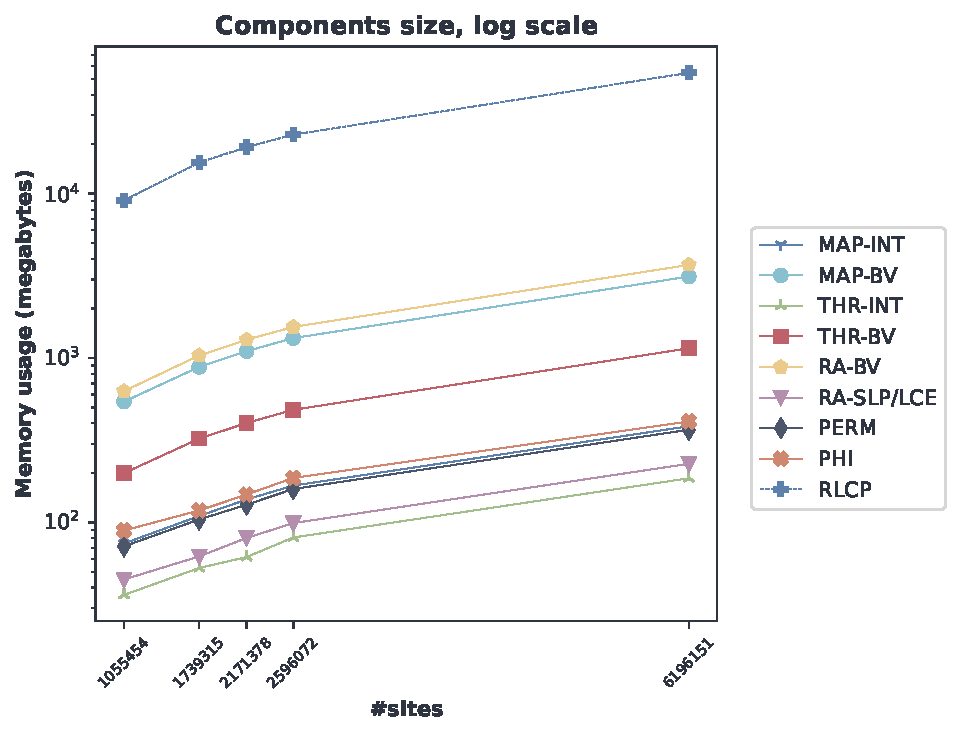
\includegraphics[width=0.8\textwidth]{img/comp_mem22.pdf}
  \end{figure}
\end{frame}
\begin{frame}{Performance costruzione strutture dati}
  \begin{figure}[H]
    \centering
    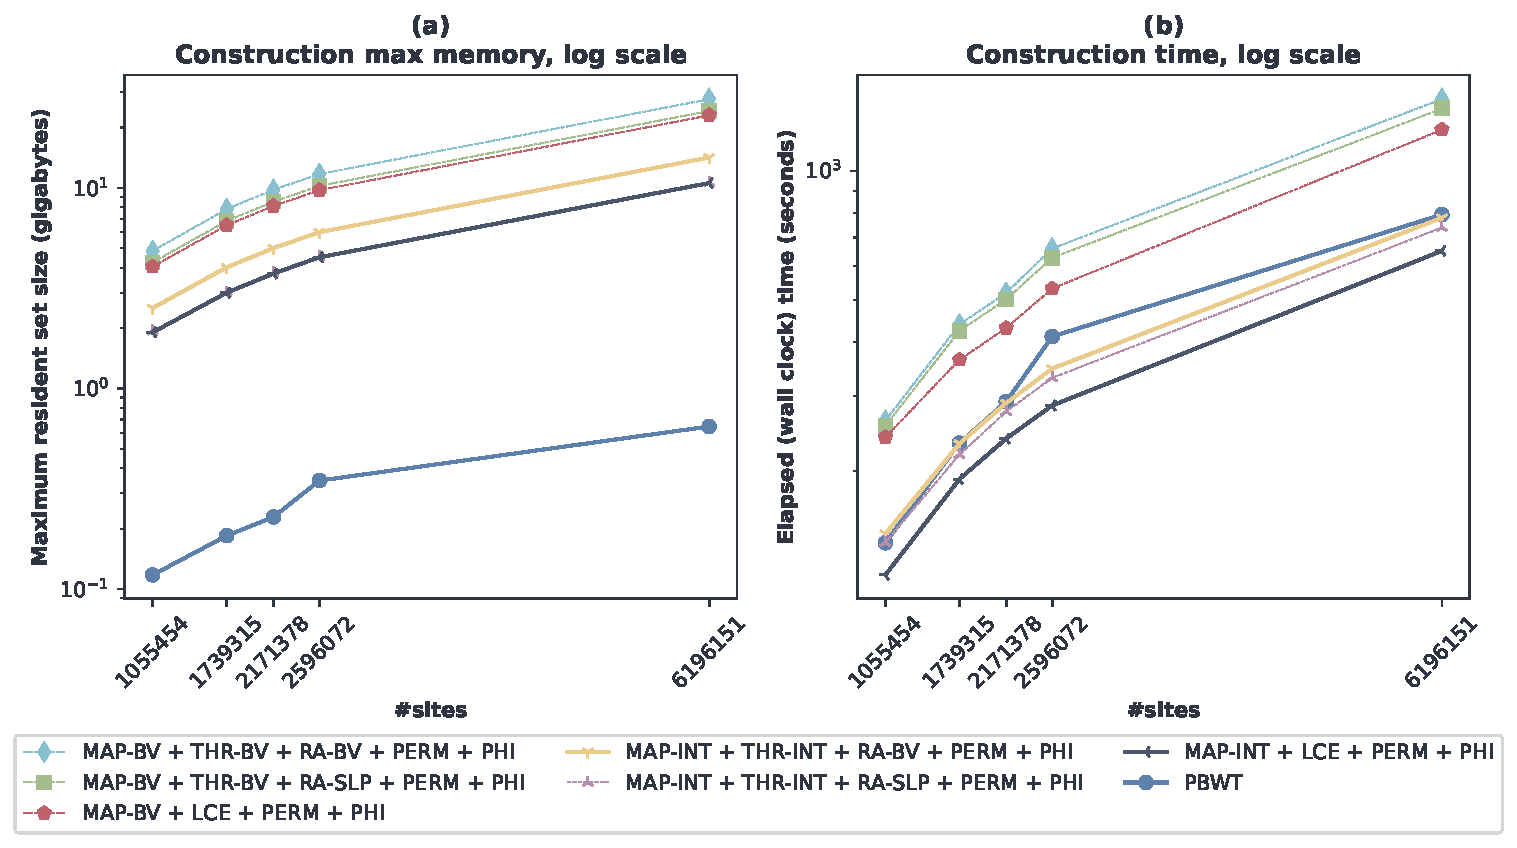
\includegraphics[width=0.99\textwidth]{img/make_time_mem_paper2.pdf}
  \end{figure}
\end{frame}
\subsection{Risultati del calcolo degli SMEM}
\begin{frame}{Performance calcolo degli $\SMEM$ con 100 query}
  \begin{figure}[H]
    \centering
    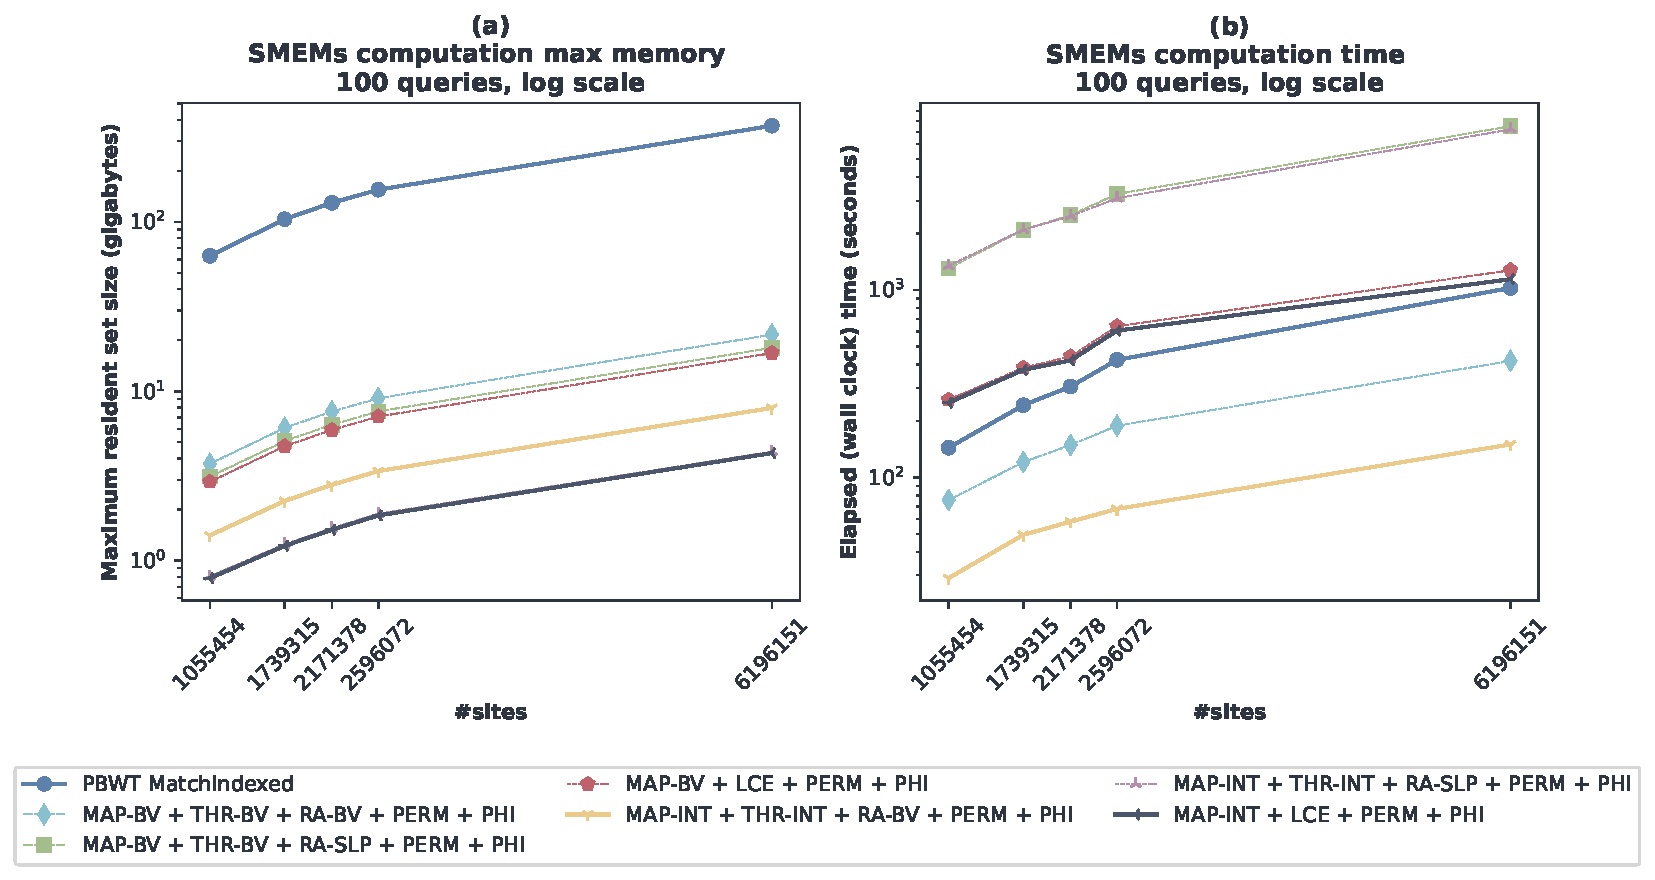
\includegraphics[width=0.99\textwidth]{img/exe_time_mem_paper2.pdf}
  \end{figure}
\end{frame}
\begin{frame}{Performance calcolo degli $\SMEM$ per singole query}
  \begin{figure}[H]
    \centering
    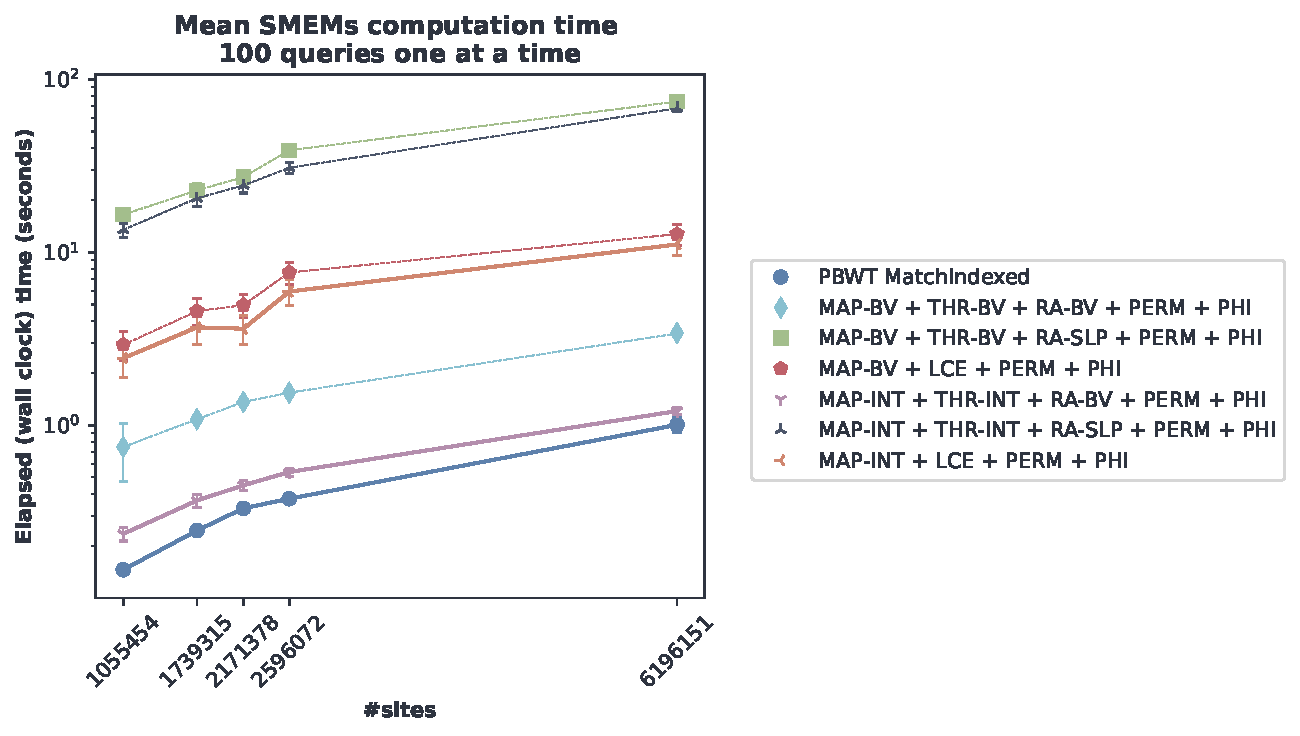
\includegraphics[width=0.99\textwidth]{img/exe_time_single_paper2.pdf}
  \end{figure}
\end{frame}
\section{Conclusioni e sviluppi futuri}
\subsection{Conclusioni e sviluppi futuri}
\begin{frame}{Considerazioni e sviluppi futuri}
  \begin{block}{Alcune considerazioni}
    \small
    \begin{itemize}
      \item le strutture dati e gli algoritmi proposti hanno
      confermato la potenzialità dell'uso di strutture run-length encoded in
      pangenomica
      \item l'obbiettivo della tesi, ovvero lo sviluppo di un algoritmo,
      efficiente in spazio, per il calcolo degli $\SMEM$ di un aplotipo esterno
      contro un pannello, è stato raggiunto con risultati molto interessanti
    \end{itemize}
  \end{block}
  \begin{block}{Sviluppi futuri}
    \small
    \begin{multicols}{2}
      \begin{itemize}
        \item ottimizzazioni per pannelli di query
        \item $\SMEM$ interni con $\RLPBWT$
        \item $\RLPBWT$ con dati mancanti
        \item $\RLPBWT$ multiallelica
        \item calcolo $\KSMEM$ con $\RLPBWT$
      \end{itemize}
    \end{multicols}
  \end{block}
\end{frame}
\begin{frame}{}
  \begin{block}{Ulteriori dettagli}
    \footnotesize{\textit{\textbf{Bonizzoni, Boucher, Cozzi, Gagie, Kashgouli,
          K\"{o}ppl e Rossi:} \\Compressed data structures for population-scale
        positional Burrows--Wheeler transforms}, {\footnotesize{bioRxiv
          (preprint), 2022}}} 
  \end{block}
  \begin{alertblock}{}
    \begin{center}
       {\LARGE{Grazie per l'attenzione}}
    \end{center}
  \end{alertblock}
  \vspace{-0.2cm}
  \begin{figure}[H]
    \centering
    
\includegraphics[scale = 0.5]{img/logo-bias-mini.png}
  \end{figure}
  \vspace{-0.3cm}
  \begin{figure}[H]
    \centering
    % 
\includegraphics[scale = 1]{img/logo_unimib.pdf}
    % 
\includegraphics[scale = 0.4]{img/ufl.png}
    % 
\includegraphics[scale = 0.25]{img/dal.png}
    % 
\includegraphics[scale = 0.15]{img/tmdu.jpg}
    
\includegraphics[width = 0.16\textwidth]{img/logo_unimib.pdf}$\quad\quad$
    
\includegraphics[width = 0.15\textwidth]{img/ufl.png}$\quad\quad$
    
\includegraphics[width = 0.16\textwidth]{img/dal.png}$\quad\quad$
    
\includegraphics[width = 0.16\textwidth]{img/tmdu.jpg}
  \end{figure}
\end{frame}
% \section{Bibliografia}
% \begin{frame}[allowframebreaks]{Bibliografia} 
%   \bibliographystyle{unsrt}
%   \bibliography{slides}
% \end{frame}
% \begin{frame}{}
%   \setbeamercolor{palette primary}{bg=nord3,fg=white}
  
%   \title[] {Grazie per l'attenzione}

%   % \subtitle
%   % {Presentation Subtitle} % (optional)

%   \author[1]{\Large{Davide Cozzi}}


%   \institute[] {\large{\textbf{{\color{nord2}Relatore:}}
%       \textit{Prof.ssa~Raffaella 
%         Rizzi}\quad 
%       \textbf{\color{nord2}{Correlatore:}} \textit{Dr.~Yuri Pirola}}\\
%     \vspace{4mm}
%     \small{\textit{Dipartimento di Informatica, Sistemistica e Comunicazione
%         (DISCo)\\
%         Università degli Studi di Milano Bicocca}}}

%   \maketitle
% \end{frame}

\end{document}


